\documentclass[11pt,reqno]{amsart}
\usepackage[T1]{fontenc}
\usepackage[utf8]{inputenc}
\usepackage{lmodern,microtype,amsmath,amssymb,amsthm,mathtools,mathrsfs}
\usepackage{graphicx,booktabs,longtable,array,xcolor,placeins}
\usepackage{tikz}
\usetikzlibrary{arrows.meta,positioning,fit,backgrounds}
\usepackage[colorlinks=true,linkcolor=blue!45!black,citecolor=blue!45!black,urlcolor=blue!45!black]{hyperref}
\hypersetup{pdftitle={Universal Support Theorems for Resilient Coverage},pdfauthor={Deep Bhattacharjee; Ushashi Bhattacharya; Sanjeevan Singha Roy}}
\usepackage[capitalise,noabbrev]{cleveref}
\setlength{\textwidth}{6.1in}
\setlength{\oddsidemargin}{.2in}
\setlength{\evensidemargin}{.2in}
\setlength{\textheight}{8.65in}
\setlength{\topmargin}{0in}
\setcounter{tocdepth}{1}
\renewcommand{\topfraction}{.9}
\renewcommand{\textfraction}{.08}
\renewcommand{\floatpagefraction}{.5}
\newtheorem{theorem}{Theorem}[section]
\newtheorem{proposition}[theorem]{Proposition}
\newtheorem{lemma}[theorem]{Lemma}
\newtheorem{corollary}[theorem]{Corollary}
\theoremstyle{definition}
\newtheorem{definition}[theorem]{Definition}
\newtheorem{example}[theorem]{Example}
\newtheorem{algorithm}[theorem]{Algorithm}
\theoremstyle{remark}
\newtheorem{remark}[theorem]{Remark}
\newcommand{\R}{\mathbb R}
\newcommand{\F}{\mathcal F}
\newcommand{\M}{\mathcal M}
\newcommand{\W}{\mathcal W}
\newcommand{\cC}{\mathcal C}
\newcommand{\cP}{\mathcal P}
\newcommand{\FF}{\mathbb F_2}
\newcommand{\abs}[1]{\left|#1\right|}
\DeclareMathOperator{\rank}{rank}
\DeclareMathOperator{\sd}{sd}
\DeclareMathOperator{\conv}{conv}
\DeclareMathOperator{\diam}{diam}
\DeclareMathOperator{\im}{im}
\DeclareMathOperator{\Max}{Max}
\DeclareMathOperator{\Min}{Min}
\title[Universal support theorems]{Universal Support Theorems for Resilient Coverage}
\author{Deep Bhattacharjee\textsuperscript{*}}
\address{Electro-Gravitational Space Propulsion Laboratory (EGSPL), Bhubaneswar, Odisha, India}
\email{itsdeep@live.com}
\urladdr{https://orcid.org/0000-0003-0466-750X}
\author{Ushashi Bhattacharya}
\address{Dortmund, Germany; National Taiwan University, Taipei, Taiwan}
\author{Sanjeevan Singha Roy}
\address{Formerly, Birla Institute of Technology (BIT) Mesra, India}
\email{sanjeevan9905@gmail.com}
\urladdr{https://orcid.org/0000-0002-6148-1421}
\date{October 28, 2026}
\subjclass[2020]{Primary 68U05; Secondary 05C65, 55U10, 90B25, 90C05}
\keywords{sensor resilience, geometric certificates, monotone failure models, critical radius, robust optimization, computational topology}
\thanks{\textsuperscript{*}First author and corresponding author: Deep Bhattacharjee, \texttt{itsdeep@live.com}.}
\begin{document}
\begin{abstract}
We prove a finite support theorem for monotone combinations of functions with a common convex part. On a compact polyhedral target, one set of points suffices to locate the maximum for every monotone rule and every common convex term. A critical point on a face of dimension $f$ needs at most $f+1$ supporting functions. For rational geometric data, the support points are rational. Applied to sensing disks, the theorem determines exact coverage radii and power thresholds for every monotone failure rule. It also gives the complete radius--failure-budget frontier from one finite construction. At a fixed geometry, the inclusion-minimal contact sets form a canonical target certificate with explicit failure witnesses. We prove exact update rules, reductions for independent geometric uncertainty and primal--dual certificates for protection allocation. Symbolic engineering examples distinguish overlap count, fault-domain resilience and protection cost. The proofs are analytical throughout. Detailed derivations, diagrams, counterexamples and appendices make the assumptions and conclusions explicit; the established geometric, topological and reliability foundations are credited.
\end{abstract}
\maketitle
\tableofcontents
\section{Introduction}
Coverage design has three logically different tasks. One must establish that a specified target is covered, determine which failures destroy that property, and choose a design or protection policy that meets a quantitative requirement. Computing the topology of the union addresses an important part of the geometry, but it does not by itself answer the target question. A contractible covered region can be disjoint from the asset that must be monitored.

This paper studies a finite model in which the geometry can be certified exactly. Physical footprints are closed disks, the target is a finite union of closed nondegenerate triangles, and failure rules are monotone with respect to additional functioning contacts. We use the model to connect a canonical geometric certificate with exact failure budgets, common-radius design, uncertainty and fault-domain assignment. Every statement below specifies its hypotheses; no physical noise distribution or hardware cost law is inferred from the geometry.

\subsection{Two reusable certificates}
For a point $x$ of the target $T$, let $S(x)$ be the set of contacts whose footprints contain $x$. Define
\begin{equation}\label{eq:overview-antichain}
\mathcal A_T=\Min\{S(x):x\in T\},
\end{equation}
where $\Min$ removes every strict superset of another member. For the regular closed targets considered here, every member has a representative away from all disk and target boundaries. A vertical-slice construction finds a rational representative for each member without approximate intersection decisions.

The first certificate is this antichain together with its witnesses. If $\F$ is any downward-closed family of allowed failures, then
\begin{equation}\label{eq:overview-universal}
T\subseteq R_{\F}\quad\Longleftrightarrow\quad
A\notin\F\text{ for every }A\in\mathcal A_T.
\end{equation}
One geometric computation therefore answers every such failure query. The antichain is the minimal-cut family of the target-coverage reliability system, rather than a new definition of a coherent system. Its geometric origin makes it possible to attach an explicit target location to each cut.

The second certificate concerns common-radius design. Fix sites and target but let all primitive disk radii equal an unknown $r$. We construct a finite set $Q_T$ of rational points, independent of the winning rule. For every monotone rule $w$ that wins on the full contact set, define
\[
\rho_w(x)=\min_{\sigma:\,w(\sigma)=1}\max_{i\in\sigma}\|x-c_i\|.
\]
Then the exact critical radius satisfies
\begin{equation}\label{eq:overview-radius}
(r_w^*)^2=\max_{q\in Q_T}\rho_w(q)^2\in\mathbb Q.
\end{equation}
The smaller support construction uses target vertices, bisector--edge intersections and three-site circumcenters, for $O(n^3+n^2h+h)$ candidates. It is valid simultaneously for all rules and all common radii. A fixed-dimensional theorem uses at most $d+1$ supporting sites on a $d$-dimensional target. We retain the larger full distance-order arrangement as an independent comparison; no optimal running-time claim is made.

\subsection{Pure mathematics, applied mathematics and engineering}
The pure mathematical part identifies the canonical antichain, proves its minimality for universal failure queries, describes its behavior under monotone label maps and relates the geometry to nerve and Dowker models. The general support theorem covers functions with a common continuous convex part and affine differences. Its finite support set works for every monotone rule and every common convex term. The radius function is a lattice polynomial in the contact distances, an established class of functions~\cite{lattice,reliability-lattice}.

The applied mathematical part gives exact arithmetic, finite algorithms, geometric uncertainty reductions and optimization certificates. For product uncertainty sets, robustification commutes with every monotone Boolean contact rule. Independent displacement balls therefore reduce exactly to disk erosion. Independent polygonal displacement sets reduce to finite intersections of disks at their vertices. Protection allocation is a linear program whose solutions are checked with rational primal and dual witnesses.

The engineering part derives complete target coverage, failure budgets, wiring choices and uncertain placement in exact symbolic examples. In the four-corner example, changing the domain assignment changes the model's coverage reliability from $81/100$ to $99/100$ at domain failure probability $1/10$, while leaving positions, radii and contact count unchanged. The exact squared radii for surviving a domain loss change from $89/25$ to $68/25$. These are analytical consequences of the stated model, not experimental performance claims about manufactured sensors.

\begin{figure}[tb]
\centering
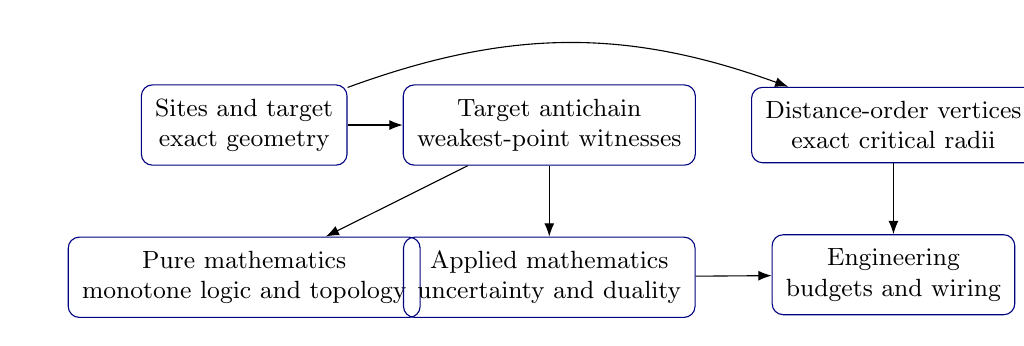
\begin{tikzpicture}[>=Latex,b/.style={draw=blue!50!black,rounded corners,align=center,font=\small,inner sep=5pt},node distance=9mm and 7mm]
\node[b] (geo) {Sites and target\\exact geometry};
\node[b,right=of geo] (cuts) {Target antichain\\weakest-point witnesses};
\node[b,right=of cuts] (radius) {Distance-order vertices\\exact critical radii};
\node[b,below=of geo] (logic) {Pure mathematics\\monotone logic and topology};
\node[b,below=of cuts] (opt) {Applied mathematics\\uncertainty and duality};
\node[b,below=of radius] (eng) {Engineering\\budgets and wiring};
\draw[->] (geo)--(cuts);\draw[->] (geo) to[bend left=20] (radius);
\draw[->] (cuts)--(logic);\draw[->] (cuts)--(opt);\draw[->] (radius)--(eng);\draw[->] (opt)--(eng);
\end{tikzpicture}
\caption{The two finite geometric certificates and their roles. Geometry is evaluated before selecting a failure rule or protection allocation.}
\end{figure}

\subsection{Relation to established work}
Arrangements of algebraic curves and exact geometric predicates are standard tools in computational geometry~\cite{arrangements}. Coverage algorithms based on circle intersections and local geometry precede this paper~\cite{integrated,coverage2003}. Homological sensor criteria and multicover nerves are likewise established~\cite{ghrist,desilva,controlled,sheehy,corbet,alonso}. We give the needed maps and proofs because the failure semantics and boundary conventions matter for the certificates.

Minimal cut sets and structure functions belong to reliability theory~\cite{barlow}. Cover decomposition and polychromatic hypergraph coloring provide the appropriate context for fault-domain assignment~\cite{polychromatic}. Max--min scalar functions built from monotone logic are lattice polynomials~\cite{lattice,reliability-lattice}; Boolean combinations of balls and generalized Voronoi decompositions also occur in the geometric work of Csik\'os~\cite{csikos}. The protection program uses ordinary linear programming duality. The treatment of uncertain geometry is situated within robust optimization~\cite{robustbook}, and marginal-only probability bounds are instances of the logical probability programs studied by Hailperin~\cite{hailperin}.

Accordingly, the contribution proposed here is the precise geometric construction and its verified synthesis, including reusable rational witnesses, exact uncertainty reductions and common-radius certificates under one failure interface. The manuscript does not claim to have discovered arrangements, minimal cuts, lattice polynomials or LP duality. Establishing priority for the full combination and assessing its significance require specialist comparison with this literature.

The earlier sensor manuscript~\cite{original} provides background for the contact-intersection model. The ECoG archive~\cite{ecog} motivates separating exact predicates, continuous target certificates and illustrations. The authors' circuit-topos, topological-deformation and linkage studies~\cite{topoi,suspension,linkage} are contextual references; none is a premise of a proof here.

\subsection{Conventions and scope}
All targets in the exact planar algorithms are finite unions of nondegenerate closed triangles with rational vertices. These targets are regular closed: $T=\overline{\operatorname{int}T}$. They may be disconnected or have holes. A wire target or an isolated point requires a lower-dimensional treatment and is excluded from the full-dimensional sampling theorem.\footnote{Regular closed does not mean convex or simply connected. The condition ensures that failure of a closed coverage set at a target boundary point is witnessed arbitrarily nearby in the target interior.}

Disk centers and radii are rational. A supplied binary64 number is treated as its exact rational value. The new target and radius routines preserve explicit \texttt{Fraction} inputs; the legacy topology routine documents its separate binary64 conversion convention. All masks retain physical contact labels, including coincident footprints. Ordinary homology is over $\FF$ unless another field is specified. The target certificates themselves do not depend on a choice of homology coefficients.

The main text develops the exact certificates and their uses. The appendices include comparison homotopies, the closed-cover chain argument, arithmetic derivations, dual certificates, worked examples and boundary counterexamples. Every mathematical conclusion in the manuscript is proved analytically. Optional software checks are supplied separately and are not premises of those proofs. Figures illustrate the arguments; no grid resolution or simulated observation determines a theorem or example.

\section{Failure families and surviving regions}
\label{sec:failures}
\begin{definition}
A \emph{failure family} is a downward-closed set $\F\subseteq2^{[n]}$ with $\varnothing\in\F$. Its complement $\W=2^{[n]}\setminus\F$ is the family of \emph{winning contact sets}. Thus $S\in\W$ and $S\subseteq S'$ imply $S'\in\W$. The active contact set at $x$ is
\[
S(x)=\{i\in[n]:x\in D_i\}.
\]
\end{definition}
The word ``winning'' refers solely to survival of the prescribed failure model. It does not encode a probability, sensor independence or a clinical performance measure.

\begin{proposition}[Pointwise failure reduction]\label{prop:pointwise}
For every $x$ the following conditions are equivalent:
\begin{enumerate}
\item $x$ remains covered after every failure $F\in\F$;
\item $S(x)\notin\F$;
\item some $\sigma\subseteq S(x)$ is a minimal member of $\W$.
\end{enumerate}
Consequently, with $D_\sigma=\bigcap_{i\in\sigma}D_i$ and $\cP_{\F}=\{\sigma\in N:\sigma\notin\F\}$,
\begin{equation}\label{eq:region-unions}
R_{\F}=\bigcup_{\sigma\in\cP_{\F}}D_\sigma
=\bigcup_{\sigma\in\Min\W}D_\sigma,
\end{equation}
where empty geometric intersections contribute nothing.
\end{proposition}
\begin{proof}
Failure of coverage at $x$ after deleting $F$ means precisely that every active contact is deleted: $S(x)\subseteq F$. If $F\in\F$, downward closure then gives $S(x)\in\F$. Conversely, if $S(x)\in\F$, the allowed choice $F=S(x)$ deletes every active contact. This proves the equivalence of the first two statements. In a finite upward-closed family every member contains a minimal member, and any set containing a winning set is winning. This proves the third equivalence and both union identities.
\end{proof}

\begin{example}[Independent failures]
For an integer $q\ge0$, let $\F_q=\{F:\abs F\le q\}$. A set wins exactly when it contains at least $q+1$ contacts. Thus $R_{\F_q}$ is the ordinary $(q+1)$-fold covered region. For $q\ge n$ it is empty.
\end{example}

\begin{example}[Weighted failure budgets]\label{ex:weighted}
Give contact $i$ a nonnegative integer failure cost $c_i$ and fix an integer budget $B\ge0$. Set
\[
\F_{c,B}=\left\{F:\sum_{i\in F}c_i\le B\right\}.
\]
Then
\begin{equation}\label{eq:weighted-rule}
S\in\W\quad\Longleftrightarrow\quad\sum_{i\in S}c_i>B.
\end{equation}
This is an adversarial deletion-cost model. It is not a statement that measurements have additive quality or that physical reliability is proportional to $c_i$. Zero-cost contacts can be deleted freely; the formula still applies. The mathematical definition also allows arbitrary nonnegative real costs; rational costs permit exact finite certificate arithmetic.
\end{example}

\begin{example}[Correlated fault domains]\label{ex:domains}
Partition contacts into labeled domains $G_1,\ldots,G_s$ and allow the loss of any $q$ complete domains. Its downward closure is
\[
\F_{G,q}=\{F:F\subseteq\textstyle\bigcup_{j\in J}G_j\text{ for some }\abs J\le q\}.
\]
If $d(S)=\{j:S\cap G_j\ne\varnothing\}$, the winning rule is
\begin{equation}\label{eq:domain-rule}
S\in\W\quad\Longleftrightarrow\quad\abs{d(S)}>q.
\end{equation}
Indeed, at most $q$ domains contain $S$ exactly when all its active domains can be deleted. The downward closure includes partial deletions, but its universal survival region equals that of the allowed complete-domain losses: any partial deletion is contained in one of those losses.
\end{example}

\begin{example}[Two-fold coverage can fail a one-domain test]
Take two identical disks and assign both contacts to one domain. Their common disk is two-fold covered. Deleting that domain leaves no coverage. If instead the two contacts belong to different domains, the same geometry survives every loss of one domain. Ordinary overlap counts and the ordinary nerve without domain labels cannot distinguish these two reliability requirements.
\end{example}

\begin{proposition}[Combining requirements]\label{prop:combining}
If $\F_1,\F_2$ are failure families, then
\[
R_{\F_1\cup\F_2}=R_{\F_1}\cap R_{\F_2},\qquad
R_{\F_1\cap\F_2}=R_{\F_1}\cup R_{\F_2}.
\]
Both union and intersection on the left are downward closed.
\end{proposition}
\begin{proof}
At each point, the first equality says that $S(x)$ belongs to neither failure family. The second says that it does not belong to both. Apply De Morgan's laws to \cref{prop:pointwise}.
\end{proof}

For a simultaneous requirement of a budget bound and a domain-loss bound one must specify whether the adversary may use either rule separately, both at once, or a composed deletion. These are different failure families. The framework accepts each, but it does not identify them without a stated model.

\begin{example}[Independence systems]
An independence system on $[n]$ is, by definition, downward closed. Taking it as $\F$ makes its dependent sets the winning coalitions. For a matroid, the minimal winning coalitions are its circuits. This observation is a translation of definitions; no matroid representation hypothesis is needed for the dual construction. The number of minimal winning coalitions can nevertheless be large, which is a reason to evaluate a winning predicate on facet intersections instead of listing all such coalitions.
\end{example}

\begin{lemma}[Monotonicity]\label{lem:monotonicity}
If $D_i\subseteq D_i'$ for every label $i$, then $R_{\F}(D)\subseteq R_{\F}(D')$. If $\F_1\subseteq\F_2$, then $R_{\F_2}(D)\subseteq R_{\F_1}(D)$.
\end{lemma}
\begin{proof}
In the first case $S_D(x)\subseteq S_{D'}(x)$ and winning is upward closed. In the second case $S(x)\notin\F_2$ implies $S(x)\notin\F_1$.
\end{proof}

\section{The canonical target antichain}
\label{sec:universal}
We first isolate a fact about closed footprints and regular closed targets. This step is what permits an exact full-target conclusion from open arrangement cells.

\begin{lemma}[Interior witnesses]\label{lem:interior-witness}
Let $T=\overline{\operatorname{int}T}$ be a nonempty regular closed target and let $D_1,\ldots,D_n$ be closed sets whose boundaries have empty interior. For every $x\in T$ there is a point $y\in\operatorname{int}T$, away from all the boundaries, with $S(y)\subseteq S(x)$. For a finite disk family and triangular target, $y$ may be chosen rational.
\end{lemma}
\begin{proof}
For each $i\notin S(x)$, closedness gives an open neighborhood of $x$ disjoint from $D_i$. Intersect these finitely many neighborhoods to obtain an open set $U$ in which no new active label can appear. Regular closedness implies $U\cap\operatorname{int}T\ne\varnothing$. A finite union of disk boundaries and target edges has empty interior, so it cannot exhaust this nonempty open set. Choose $y$ outside it. The active labels of $y$ are all in $S(x)$. In the disk setting, the remaining open set contains rational points by density of $\mathbb Q^2$.
\end{proof}

For the first general statement, the avoidance assertion uses that the finitely many boundaries are closed with empty interior, hence nowhere dense. Disk circles and target edges satisfy this condition. No claim about arbitrary nonclosed sensing footprints is needed.

\begin{definition}
The \emph{target antichain} is
\[
\mathcal A_T(D)=\Min\{S(x):x\in T\}.
\]
The empty contact set is retained if realized. If it occurs, it is the unique minimal member. A witness for $A\in\mathcal A_T$ is a point $q_A\in T$ with $S(q_A)=A$.
\end{definition}

\begin{theorem}[Universal target certificate]\label{thm:universal}
For a finite closed-disk family and a regular closed triangular target, $\mathcal A_T$ is exactly the collection of inclusion-minimal labels of the two-dimensional target arrangement cells. Every member has a rational interior witness. For every downward-closed failure family $\F$ containing the empty set,
\begin{equation}\label{eq:universal-target}
T\subseteq R_{\F}\quad\Longleftrightarrow\quad
\mathcal A_T\cap\F=\varnothing.
\end{equation}
If $h$ target-edge segments are supplied, the certificate has $O((n+h)^2)$ members.
\end{theorem}
\begin{proof}
The finite collection of all realized masks has an inclusion-minimal member below every mask. If $A$ is such a minimal mask, apply \cref{lem:interior-witness} at a point realizing $A$. The resulting interior mask is a subset of $A$, so minimality forces equality. Conversely, if an interior-cell mask is minimal among interior-cell masks, a smaller realized mask would have an interior witness below it by the lemma, a contradiction. Thus the two minimal collections agree.

By \cref{prop:pointwise}, full target coverage means $S(x)\notin\F$ for every $x\in T$. Necessity of the right side is immediate from witnesses. For sufficiency, choose $A\subseteq S(x)$ in the antichain. If $S(x)\in\F$, downward closure would imply $A\in\F$, contradicting the right side. This proves \cref{eq:universal-target}.

For the size bound, refine the disk arrangement by the supporting lines of all target edges. With $n$ distinct positive-radius circles, adding circle $j$ creates at most $\max\{1,2(j-1)\}$ new regions. A newly added line meets the circles at most $2n$ times and the preceding $j-1$ lines at most $j-1$ times, so it creates at most $2n+j$ regions. Coincident curves can be removed for counting; repeated sensor labels are still preserved on each region. Zero-radius disks add no two-dimensional region. Consequently the total number of regions is at most
\begin{equation}\label{eq:arrangement-bound}
n^2-n+2+2nh+\frac{h(h+1)}2,
\end{equation}
where the harmless initial constant also bounds the $n=0$ case. Target membership and contact labels are constant on every open region of this refined arrangement. The number of minimal labels cannot exceed its number of regions.
\end{proof}

\begin{remark}
The quadratic bound counts the retained certificate, not the vertical bands sampled in its construction. It is inherited from ordinary arrangement complexity. No matching quadratic lower bound for this particular minimal-label family is asserted.
\end{remark}

\begin{proposition}[Irredundancy for all failure rules]\label{prop:irredundant}
Every member of $\mathcal A_T$ is necessary if a certificate consists of realized contact masks and is required to answer all downward-closed failure queries by testing those masks. In particular, deleting any one member can change an answer.
\end{proposition}
\begin{proof}
Fix $A\in\mathcal A_T$ and use $\F=2^A$. Then $A$ loses. Every other antichain member $B$ is not a subset of $A$, so $B\notin\F$. Testing all the remaining members would therefore accept although the witness $q_A$ fails. When $A=\varnothing$, its antichain has only that member and the same argument applies to the family allowing only the empty failure, $2^\varnothing=\{\varnothing\}$.
\end{proof}

This is minimality of the representation by realized masks. It is not a lower bound against every possible compressed circuit, geometric formula or data structure.\footnote{An irredundant list can still admit a shorter symbolic representation. We do not identify the number of listed cuts with an information-theoretic lower bound for all encodings.}

\begin{theorem}[Monotone relabeling]\label{thm:relabel}
Let $\gamma:2^{[n]}\to2^{[m]}$ preserve inclusion. The minimal target patterns after applying $\gamma$ to active sets are exactly
\begin{equation}\label{eq:relabel}
\Min\{\gamma(A):A\in\mathcal A_T\}.
\end{equation}
Each retained image inherits a witness from its preimage. Thus no new geometric computation is needed for contact deletion, fault-domain coarsening or monotone virtual-contact logic.
\end{theorem}
\begin{proof}
Every realized $S(x)$ contains some $A\in\mathcal A_T$, so $\gamma(S(x))$ contains $\gamma(A)$. Conversely every image $\gamma(A)$ is itself realized at $q_A$. Taking minimal members on both sides proves the equality and the witness assertion.
\end{proof}

For a permanent deletion set $F$, take $\gamma(S)=S\setminus F$. For a partition into domains, take $\gamma(S)$ to be the set of domains touched by $S$. For a contact represented by several primitive disk constraints, let its output bit be one exactly when all its primitive bits are one. This conjunction map is monotone and is used for uncertain placement in \cref{sec:uncertainty}.

\begin{corollary}[Exact deletion budgets]\label{cor:budgets}
For nonnegative contact deletion costs $c_i$, the minimum cost of a failure that destroys full target coverage is
\begin{equation}\label{eq:kappa}
\kappa_T(c)=\min_{A\in\mathcal A_T}\sum_{i\in A}c_i.
\end{equation}
It is attained by deleting a minimizing $A$, with failure witnessed at $q_A$. Full target coverage survives every deletion of cost at most $B$ if and only if $B<\kappa_T(c)$.
\end{corollary}
\begin{proof}
A deletion $F$ destroys coverage precisely when it contains a realized active set, and hence when it contains some antichain member. Nonnegative costs give $c(F)\ge c(A)$. Conversely deleting $A$ removes every active contact at its witness. The strict budget inequality follows because a deletion of cost exactly $\kappa_T(c)$ is allowed when $B$ reaches that value.
\end{proof}

For unit costs, the maximum guaranteed number of arbitrary contact losses is $\min_A|A|-1$, provided the target is initially covered. For a domain partition, apply \cref{thm:relabel} first and use one cost per domain. The case $\kappa_T=0$ is not rounded up: it means that no nonnegative budget guarantee holds, either because the target is already uncovered or because a zero-cost cut is available.

\begin{figure*}[tb]
\centering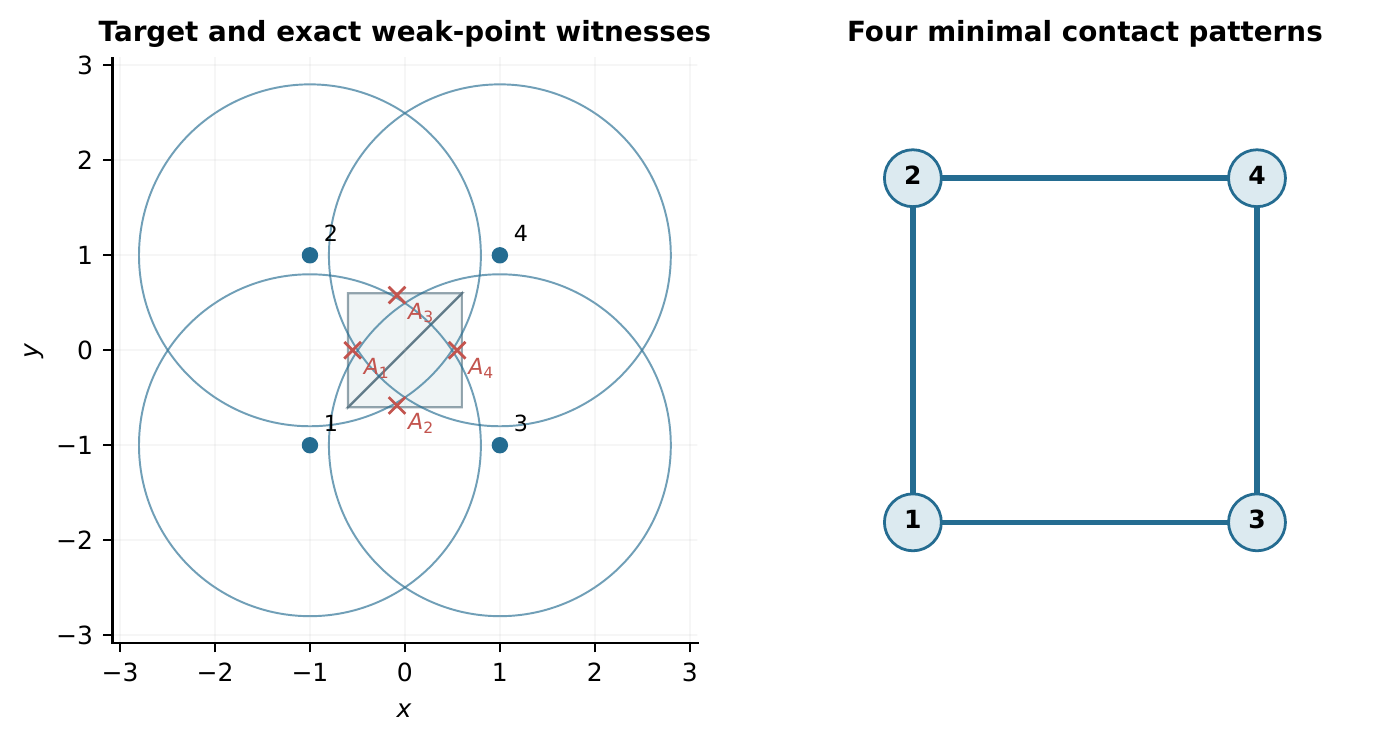
\includegraphics[width=\textwidth]{figures/target-patterns.png}
\caption{Target geometry with exact rational witnesses and the minimal cut graph of the four-contact panel. The witnesses and all four critical pair patterns are derived explicitly in \cref{sec:engineering}.}
\end{figure*}


\section{An exact construction with rational target witnesses}
\label{sec:target-algorithm}
We now construct the certificate of \cref{thm:universal}. The implementation deliberately uses a transparent vertical-slice method rather than an optimal arrangement data structure. Its witness list can be checked using rational point membership alone.

\subsection{Critical abscissae}
Include the following real numbers in a list $X$:
\begin{enumerate}
\item the first coordinates of every target vertex;
\item the leftmost and rightmost first coordinates $c_{i,x}\pm r_i$ of each disk;
\item the first coordinates of every intersection of two distinct supporting circles;
\item the first coordinates of every intersection of a circle with a target-edge segment;
\item the first coordinates of every intersection of two target-edge segments.
\end{enumerate}
Remove duplicates and numbers outside the horizontal span of the target. Pairwise coincidences create no infinite list: coincident circle boundaries are represented once for ordering, while contact labels remain distinct; overlapping collinear segments need only their endpoints. Their order does not exchange inside an open slab.

There are $O((n+h)^2)$ listed numbers. Each is rational or has the form $a+b\sqrt d$ with $a,b,d\in\mathbb Q$ and $d\ge0$. Circle--circle formulas are derived in \cref{sec:geometry}. For a segment $p+t(q-p)$, circle intersection is a quadratic equation in $t$, retaining roots in $[0,1]$. Segment intersections have rational coordinates.

For each consecutive pair $\alpha<\beta$ in $X$, choose a rational $x_0\in(\alpha,\beta)$. The vertical line at $x_0$ meets a circle, when appropriate, at
\[
y=c_{i,y}\pm\sqrt{r_i^2-(x_0-c_{i,x})^2},
\]
and a nonvertical target edge at a rational ordinate. Sort these ordinates exactly, remove duplicate values and choose a rational ordinate between every consecutive pair. Test the resulting point for membership in the target interior and, if retained, compute its exact contact mask.

The target is bounded, so every interior component of its vertical section is bracketed by target-edge intersections. Sampling the two unbounded ordinate intervals is unnecessary. Vertical target edges lie on critical abscissae; their omission from generic sections is justified by \cref{lem:interior-witness}, rather than by assuming they have no target points.

\begin{theorem}[Completeness of vertical sampling]\label{thm:sweep}
The construction visits a point in every two-dimensional arrangement cell that meets the target interior. After taking inclusion-minimal contact masks, it returns exactly $\mathcal A_T$ with rational witnesses. It also applies to any fixed monotone activation map $\gamma$, returning the minimal mapped masks.
\end{theorem}
\begin{proof}
Between consecutive critical abscissae, no circle appears or disappears in a vertical section, no target-edge segment begins or ends, and two section curves cannot exchange their order. Such an exchange would require an intersection whose first coordinate belongs to $X$. Equal section curves can persist, as with coincident circles or overlapping segments; keeping one ordinate for a persistent equality leaves every open band represented.

Thus each open ordinate band continues through the slab without a boundary crossing, and its contact labels and target membership are constant. Choosing one rational point per band gives those labels exactly. Conversely every two-dimensional target cell has an open horizontal projection, which cannot be contained in the finite list $X$. It therefore meets some open slab and one of its bands. Its mask is among the samples. \Cref{thm:universal} identifies the minimal masks with $\mathcal A_T$. For an activation map, apply \cref{thm:relabel}, or evaluate that map on every sample before minimalization.
\end{proof}

\subsection{Comparing two quadratic numbers}
Numerical square roots are not needed even to sort the critical coordinates. Let
\[
x=a+b\sqrt h,\qquad y=c+d\sqrt k,\qquad h,k\ge0.
\]
Set $A=a-c$, $U=A+b\sqrt h$ and $V=d\sqrt k$. We seek the sign of $U-V$.

\begin{lemma}[Two-radical comparison]\label{lem:two-radicals}
The sign of $x-y$ is obtained using rational arithmetic and the one-radical sign test of \cref{lem:sign}. If $U$ and $V$ have different signs, their order follows from those signs. If both are zero, the difference is zero. If their common sign is $s\in\{-1,1\}$, then
\begin{equation}\label{eq:two-radical-comparison}
\operatorname{sgn}(x-y)=s\,\operatorname{sgn}\left(A^2+b^2h-d^2k+2Ab\sqrt h\right).
\end{equation}
\end{lemma}
\begin{proof}
The cases with different signs or both zero are immediate. When $U,V$ are both positive, squaring preserves their order, and $U^2-V^2$ is the expression in parentheses. When both are negative, their order is the reverse of the order of their squares. This gives the factor $s$ and proves the formula, including equality. The sign of $U$ uses one radical, and the sign of $V$ is the sign of $d$ unless $k=0$.
\end{proof}

This test detects equal values with different representations, such as $\sqrt8=2\sqrt2$. It avoids an interval-refinement loop that would never separate two equal algebraic numbers.\footnote{The comparator is a Boolean exactness component, not a numerical approximation routine. An approximate coordinate may still be used for plotting after its role in the certificate has been completed.}

\subsection{Constructing a rational point between algebraic endpoints}
For $h=p/q\ge0$ and an integer precision $b\ge1$, compute
\[
m=\left\lfloor\sqrt{\left\lfloor\frac{p2^{2b}}q\right\rfloor}\right\rfloor.
\]
Then $m/2^b\le\sqrt h<(m+1)/2^b$, unless exact equality holds at the lower endpoint, which is checked by squaring integers. Multiplication by the signed rational coefficient and addition of the rational part give an enclosing rational interval for $a+b'\sqrt h$.

For two strictly ordered endpoints, refine their enclosures until the upper endpoint of the left enclosure is less than the lower endpoint of the right enclosure. Their rational midpoint is the desired sample. The enclosures shrink to distinct real numbers, so the process terminates. All comparisons certifying the selected point are exact. The same routine is used for horizontal and vertical samples.

\begin{proposition}[Operation counts and retained size]\label{prop:sweep-complexity}
Put $M=n+h$. The stated construction has $O(M^2)$ critical abscissae, examines $O(M^3)$ ordinate bands and retains $O(M^2)$ distinct inclusion-minimal masks. Its direct target and contact labeling implementation uses $O(M^4)$ rational predicate operations, apart from algebraic sorting and rational separation costs. The latter sorting uses $O(M^3\log M)$ comparisons of quadratic numbers.
\end{proposition}
\begin{proof}
The event count follows from pairwise circle and segment intersections and endpoint counts. Each slab has at most $2n+h=O(M)$ section ordinates, yielding the band count and sorting count. A band sample is checked against $O(h)$ triangles and $n$ contacts, giving the direct labeling bound. At most $O(M^2)$ distinct region labels are needed by \cref{eq:arrangement-bound}, and pairwise inclusion filtering of that many labels takes $O(M^4)$ mask comparisons. The claimed retained size is the canonical certificate bound, independent of how many times one region is sampled.
\end{proof}

These are operation counts, not constant-bit-time claims. Integer sizes and the number of dyadic refinement steps matter. We do not claim an optimal arrangement algorithm or a new algebraic root-separation theorem. The important guarantee is finite exactness, with a small retained certificate and a rational witness for every retained mask.

\subsection{Independent verification of a returned failure}
A rejected query supplies $A$ and $q_A$. A checker can verify that $q_A\in T$, evaluate all rational squared distances to recover $S(q_A)=A$, and confirm $A\in\F$. This independently verifies failure of the query without trusting the geometric sweep. Acceptance additionally requires completeness of the sample construction, which is supplied by \cref{thm:sweep}; checking a few returned witnesses alone cannot prove completeness.

Deleting every contact in $A$ gives a concrete adversarial failure. For a domain cut, the returned location has the mapped active-domain set recorded in the certificate. For a virtual-contact bundle, the checker evaluates the finite conjunctions at that same point. The location is therefore linked to the actual model rather than to a missing cell in a plot.

\begin{figure}[!htbp]
\centering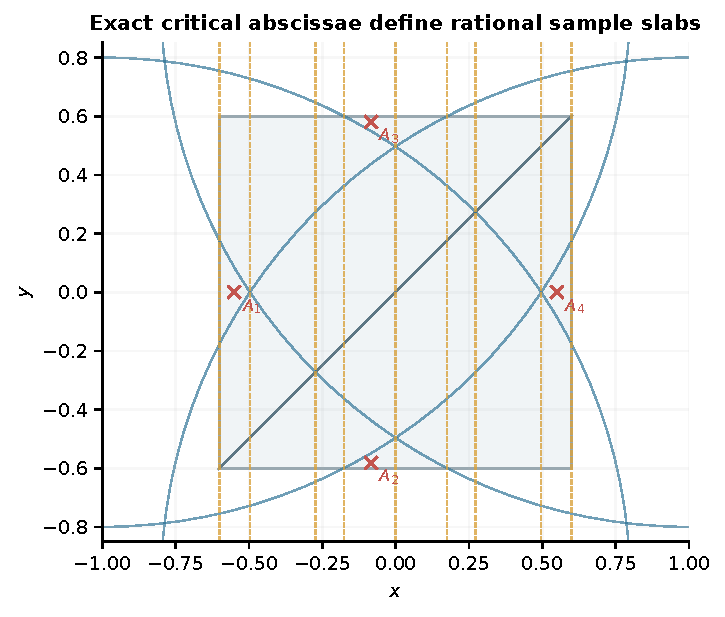
\includegraphics[width=\textwidth]{figures/vertical-slices.pdf}
\caption{Critical abscissae for the same panel. Open slabs contain no geometric ordering event. Rational samples between exact boundary ordinates recover the minimal contact labels without a raster resolution parameter.}
\end{figure}

\FloatBarrier

\section{A universal exact common-radius certificate}
\label{sec:radius}
The fixed-radius antichain answers many failure rules at one geometry. This section fixes the sites and target and determines the exact common radius needed for any one of those rules. All sites share the same radius in this theorem. Unequal-radius targets are handled by \cref{thm:sweep}, but the bisector proof below must not be applied unchanged to additive weighted distances.

Let $w:2^{[n]}\to\{0,1\}$ be monotone, with $w(\varnothing)=0$ and $w([n])=1$. Define
\begin{equation}\label{eq:required-radius}
\rho_w(x)=\min_{\sigma:\,w(\sigma)=1}\max_{i\in\sigma}\|x-c_i\|.
\end{equation}
This is the smallest common radius for which the active contact set at $x$ wins. It is a finite minimum of finite maxima of distance functions, so it is continuous and $1$-Lipschitz. The same maximum--minimum algebra underlies lattice-polynomial descriptions of reliability systems~\cite{lattice,reliability-lattice}.

\begin{lemma}[Prefix evaluation]\label{lem:prefix}
Order the squared site distances at $x$, adding every tied group together. The first prefix on which $w$ wins has maximum squared distance $\rho_w(x)^2$.
\end{lemma}
\begin{proof}
At squared radius $s$, the active set is exactly the union of all distance groups at most $s$. Before its first winning prefix, no winning subset can be contained in that active set. At the first winning prefix, the prefix itself is a winning coalition. This is exactly the minimization in \cref{eq:required-radius}.
\end{proof}

Let $\mathscr L$ contain all nontrivial perpendicular bisectors of pairs of sites and the supporting lines of all target edges. Coincident sites give no bisector; coincident lines are stored once. Let $Q_T$ contain all target vertices and every intersection of two nonparallel lines in $\mathscr L$ that lies in $T$.

\begin{theorem}[An elementary arrangement certificate]\label{thm:master-radius}
For rational sites and a triangular target,
\begin{equation}\label{eq:master-radius}
r_w^*:=\min\{r\ge0:T\subseteq R_w(r)\}
=\max_{q\in Q_T}\rho_w(q).
\end{equation}
The candidate set $Q_T$ is independent of $w$, has rational coordinates and has at most $O((n^2+h)^2)$ points. In particular $(r_w^*)^2\in\mathbb Q$. A maximizing point is an exact target witness showing that every smaller common radius fails.
\end{theorem}
\begin{proof}
The perpendicular bisectors divide the plane into cells on which the weak ordering of distances to the sites is fixed. Identical sites remain tied everywhere; there is no need to break such a tie geometrically. The additional target-edge lines subdivide every target triangle into bounded convex polygons. On the interior of one such polygon, \cref{lem:prefix} selects one fixed distance group, so $\rho_w(x)$ equals $\|x-c_j\|$ for a fixed representative site $c_j$ in that group.

The norm function is convex. Every point of the polygon is a convex combination of its vertices, and its distance to $c_j$ is at most the corresponding convex combination of vertex distances. Thus the maximum on the polygon is attained at a vertex. By continuity of $\rho_w$, the formula obtained in its interior extends to its boundary even when new distance ties occur there. Every polygon vertex is either a target vertex or an intersection of two lines in $\mathscr L$, hence belongs to $Q_T$. Taking the maximum over the finitely many target polygons proves that $\max_T\rho_w=\max_{Q_T}\rho_w$.

Coverage at common radius $r$ is equivalent to $r\ge\rho_w(x)$ at every target point by definition, giving \cref{eq:master-radius}. There are at most $\binom n2+h$ lines and a quadratic number of their pairwise intersections. Rational line coefficients give rational intersection coordinates. Squared distances at those points are rational, and \cref{lem:prefix} selects one of them. Their finite maximum is rational. A maximizing point fails at any smaller radius, proving the witness assertion.
\end{proof}

\begin{remark}[Universality and complexity]
The same $Q_T$ works for cardinality thresholds, weighted budgets, domain rules and any fixed monotone activation of primitive contacts. It does not say that the critical radius is the same for those rules. Its point is reusability and an exact threshold; specialised higher-order or coloured Voronoi methods can be faster for a single rule.
\end{remark}

\subsection{The support reduction in fixed dimension}
The full line arrangement contains many vertices created by distance ties that are irrelevant to a given threshold. A local maximum argument removes them simultaneously for every monotone rule. We state the argument in $\R^d$ to make the supporting geometry explicit.

For a finite union of rational nondegenerate $d$-simplices, construct a set $Q_T^{\mathrm{supp}}$ as follows. Include every simplex vertex. For each $f$-dimensional face $G$ of each simplex, with $1\le f\le d$, and each choice of $f+1$ sites, solve the $f$ equations asserting equal squared distance to those sites, restricted to the affine hull of $G$. Retain the solution if it is unique and lies in $G$. All these equations are linear after subtracting one squared-distance equation from the others.

\begin{theorem}[Universal support certificate]\label{thm:support-radius}
For every monotone rule $w$ with $w(\varnothing)=0$ and $w([n])=1$,
\begin{equation}\label{eq:support-radius}
r_w^*=\max_{q\in Q_T^{\mathrm{supp}}}\rho_w(q).
\end{equation}
The set is independent of $w$, has rational coordinates, and for $t$ supplied simplices has size at most
\begin{equation}\label{eq:support-count}
t(d+1)+t\sum_{f=1}^d\binom{d+1}{f+1}\binom n{f+1}.
\end{equation}
In particular, for fixed dimension it has $O(t(1+n^{d+1}))$ points, and $(r_w^*)^2$ is rational.
\end{theorem}
\begin{proof}
Choose a maximizer $x$ of the continuous function $\rho_w$ on $T$. Choose one target simplex containing $x$, and let $G$ be its unique face whose relative interior contains $x$. Write $f=\dim G$. If $f=0$, $x$ is a supplied vertex and is already in the certificate.

Suppose $f\ge1$. Let $s=\rho_w(x)$, let $L$ contain the sites strictly closer than $s$, and let $J$ contain those at distance exactly $s$. By \cref{lem:prefix}, $w(L)=0$ and $w(L\cup J)=1$. There is a neighborhood of $x$ in which all sites of $L$ remain closer than all sites of $J$, and all other sites remain farther than all sites of $J$.

Fix $j_0\in J$. Consider the linear functionals $v\mapsto(c_j-c_{j_0})\cdot v$ on the $f$-dimensional tangent space of $G$. If they have rank less than $f$, choose a nonzero tangent vector $v$ annihilated by all of them. Along $x+uv$ all distances to sites in $J$ remain equal: their squared-distance differences are zero at $u=0$ and have zero linear coefficient. For sufficiently small positive and negative $u$, the order separation from $L$ and the farther sites persists, and $x+uv$ stays in $G$. The winning threshold is therefore the common distance to $J$.

Its square along this line is
\[
\|x+uv-c_{j_0}\|^2
=s^2+2u\,v\cdot(x-c_{j_0})+u^2\|v\|^2.
\]
Since $v\ne0$, at least one of two sufficiently small opposite nonzero values of $u$ makes this strictly larger than $s^2$. This contradicts maximality of $x$.

The functionals thus have rank $f$. Choose $f$ independent ones, corresponding to $f$ sites in $J$ together with $j_0$. Their equal-distance equations have a unique solution in the affine hull of $G$, namely $x$. This is one of the retained support points. Consequently a global maximizer lies in the certificate, proving \cref{eq:support-radius}. The count enumerates the faces and site subsets; singular systems can only reduce it. Unique solutions of rational linear systems are rational, and \cref{lem:prefix} again makes the squared threshold rational.
\end{proof}

\begin{corollary}[Three-site planar construction]\label{cor:three-site}
In the plane it suffices to retain target vertices, intersections of site-pair bisectors with target-edge segments, and circumcenters of noncollinear site triples that lie in the target. The size is $O(n^3+n^2h+h)$.
\end{corollary}
\begin{proof}
The $f=1$ systems are bisector--edge intersections; a bisector coinciding with an edge does not have full rank and contributes no isolated solution. The $f=2$ systems are the circumcenters of noncollinear triples. There are at most $\binom n2$ bisectors and $h$ edges, at most $\binom n3$ circumcenters and $O(h)$ supplied vertices.
\end{proof}

The full arrangement construction provides a second analytical construction of a valid support set. The support theorem gives the smaller main construction. Its proof treats arbitrary monotone rules, not only the $k$th-nearest distance.

\begin{corollary}[One support set for every common radius]\label{cor:all-radii}
For each $r\ge0$,
\begin{equation}\label{eq:antichain-support}
\mathcal A_T(r)=\Min\{S_r(q):q\in Q_T^{\mathrm{supp}}\}.
\end{equation}
Thus a single rational support set recovers the exact target antichain at every common radius and answers every monotone failure query there. The same statement holds after a monotone activation map.
\end{corollary}
\begin{proof}
For any downward-closed family $\F$, let $w$ be its complement. If $w([n])=0$, no contact set can win and both the target and the support set fail. Otherwise \cref{thm:support-radius} says that winning at all support points at radius $r$ is equivalent to winning throughout $T$. The two collections of realized masks therefore have identical answers to every failure-family query. Their minimal antichains must coincide: if a true minimal pattern $A$ had no sampled pattern contained in it, the query $\F=2^A$ would accept all samples and fail at $A$. Conversely every sampled mask is realized in $T$ and contains a true minimal pattern. This proves \cref{eq:antichain-support}. Composition with an activation map preserves monotonicity, giving the last assertion.
\end{proof}

Support witnesses can lie on the target boundary. The vertical algorithm instead supplies interior witnesses for the same minimal masks. Either is a valid rational target witness; their roles must not be confused with merely checking a finite grid chosen without a completeness theorem.

\subsection{Exact line arithmetic}
The bisector of $c_i$ and $c_j$ is
\[
2(c_j-c_i)\cdot x+\|c_i\|^2-\|c_j\|^2=0.
\]
Represent a line by its rational coefficients $(a,b,c)$ in $ax+by+c=0$. Clearing denominators, dividing by the common integer divisor and choosing the first nonzero coefficient positive gives a canonical representation. For two lines $(a,b,c)$ and $(d,e,f)$ with determinant $\Delta=ae-db\ne0$, their intersection is
\[
x=\frac{bf-ec}{\Delta},\qquad y=\frac{cd-fa}{\Delta}.
\]
Every candidate membership test in a closed triangle is a rational orientation test. Every distance-prefix comparison uses rational squared distances. Consequently the radius computation uses no radical comparison; radicals appear only when displaying the final radius as $\sqrt s$.

\subsection{A reusable engineering example}
Take the four sites $(\pm1,\pm1)$ and target $[-3/5,3/5]^2$. Two-contact coverage requires squared radius $68/25$. Assigning both contacts in each column to the same failure domain requires squared radius $89/25$ to survive a domain loss. Assigning the two diagonals as the domains instead requires $68/25$. The saved rational worst points include $(-3/5,0)$ for column wiring and a target corner for diagonal wiring.

These values are derived directly in \cref{app:worked}. The separation is operational: a nominal radius $9/5$ lies between the two thresholds. At that radius, diagonal wiring meets the one-domain-loss requirement and column wiring fails, although ordinary two-contact coverage is identical in both designs.

\subsection{Why unequal offsets require a different proof}
If contact $i$ has radius $r_i+s$ with a common additive design variable $s$, the relevant scalar functions are $\|x-c_i\|-r_i$. Their equality loci are generally hyperbolas, not the perpendicular bisectors used here. A distance-order arrangement for the unweighted sites would then omit changes in the active ranking. The exact fixed-radius sweep still applies after the radii are chosen, and a general semialgebraic optimization approach is possible, but the rational threshold statement of this section does not cover that weighted problem.\footnote{The fixed-geometry sweep accepts unequal radii; only the radius theorem assumes a common radius.}

\begin{figure*}[tb]
\centering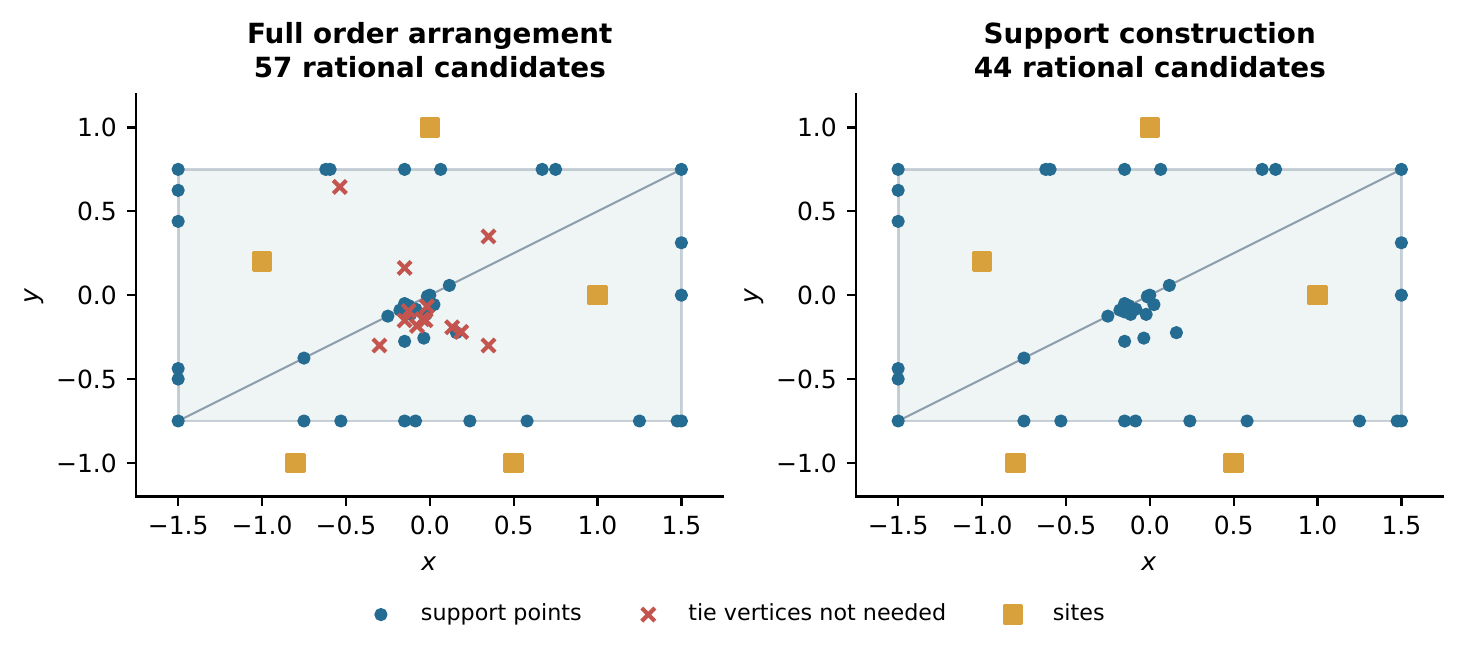
\includegraphics[width=\textwidth]{figures/support-comparison.png}
\caption{Two support constructions for five sites (gold squares) on the same two-triangle target. Left: the full distance-order arrangement, $57$ candidate points. Right: the support set of \cref{thm:support-radius}, $44$ points, valid for every monotone rule; the red crosses mark tie points of the arrangement that it does not need.}
\end{figure*}

\begin{figure*}[tb]
\centering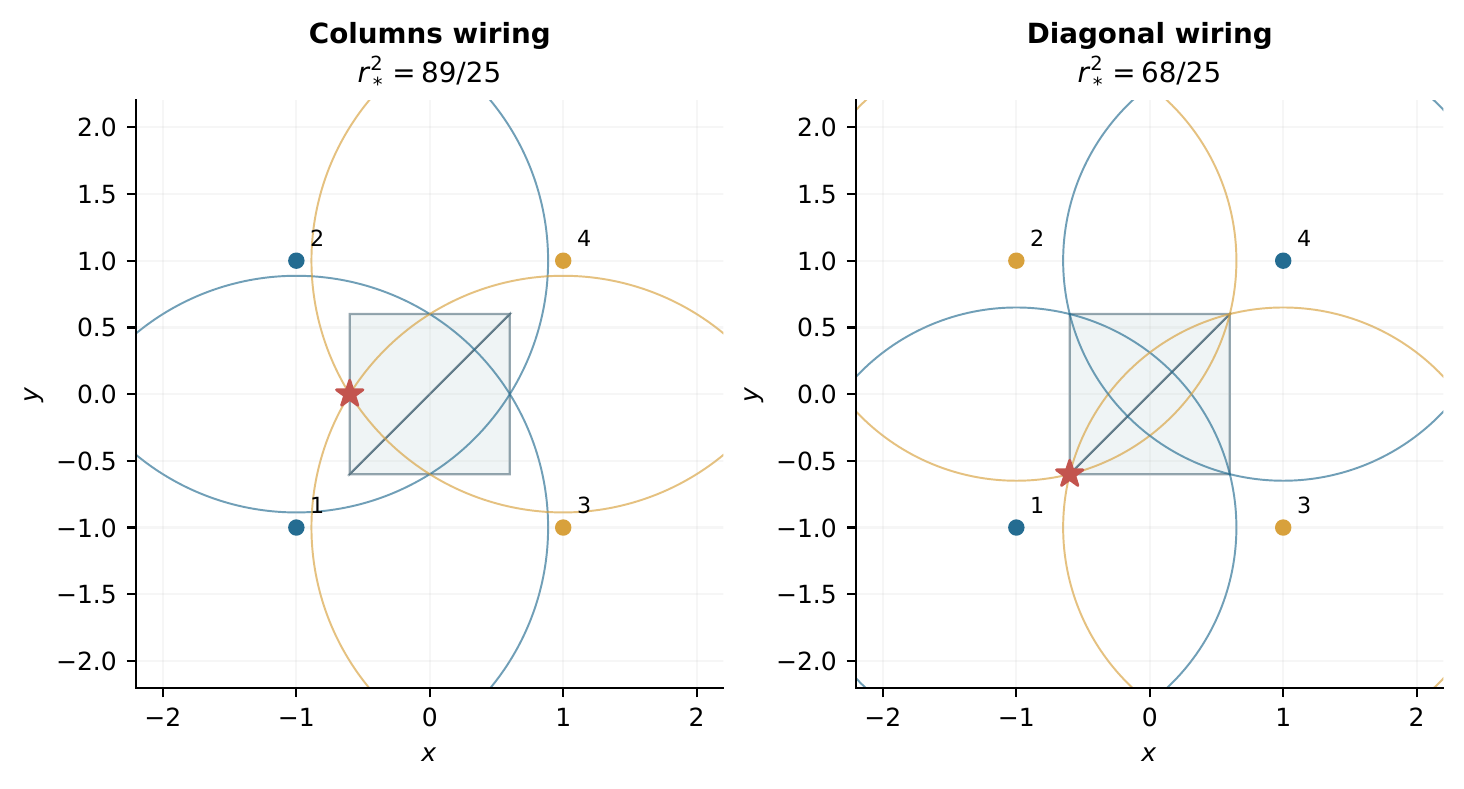
\includegraphics[width=\textwidth]{figures/radius-supports.png}
\caption{Exact critical-radius witnesses for the two wiring choices. Stars mark maximizing target locations. The circles are drawn at the certified threshold radii, whose squares are rational.}
\end{figure*}


\section{Common convex parts and exact resilience frontiers}
\label{sec:power-frontier}
The support argument does not depend on the distance functions themselves. What it uses is a common convex part and affine differences. This gives a more general analytical theorem and an exact two-parameter consequence for coverage design.

\subsection{A support theorem for lattice selectors}
Let $T$ be a finite union of nondegenerate $d$-simplices. Suppose $\psi$ is continuous and convex on every supplied simplex, and define
\begin{equation}\label{eq:common-convex}
f_i(x)=\psi(x)+a_i\cdot x+b_i,\qquad i\in[n].
\end{equation}
For a monotone rule $w$ with $w(\varnothing)=0$ and $w([n])=1$, set
\begin{equation}\label{eq:lattice-selector}
L_w(f)(x)=\min_{\sigma:\,w(\sigma)=1}\max_{i\in\sigma}f_i(x).
\end{equation}
This is a lattice polynomial without added constant arguments. Its value is one of the input values at every point. It commutes with a common additive shift of all those values. These elementary properties follow directly from the finite minimum and maximum operations.

Construct $Q_T(a,b)$ by including all target vertices and, on each $s$-dimensional simplex face, the unique solutions of $s$ independent equations
\begin{equation}\label{eq:affine-ties}
(a_{i_j}-a_{i_0})\cdot x+b_{i_j}-b_{i_0}=0,
\qquad j=1,\ldots,s,
\end{equation}
that lie in that face. The set depends on the affine data and target, but not on $w$ or $\psi$.

\begin{theorem}[Universal support for a common convex part]\label{thm:convex-support}
For every family \cref{eq:common-convex} and every nonconstant monotone rule,
\begin{equation}\label{eq:convex-support}
\max_{x\in T}L_w(f)(x)=\max_{q\in Q_T(a,b)}L_w(f)(q).
\end{equation}
The same support set works simultaneously for every continuous common convex part $\psi$, every such rule and every level threshold. Its size satisfies \cref{eq:support-count}. If the target and affine data are rational, all support points are rational.
\end{theorem}
\begin{proof}
First suppose that $\psi$ is strictly convex on every nontrivial segment of every simplex. Let $x$ maximize $L_w(f)$ and lie in the relative interior of a target face $G$ of dimension $s$. If $s=0$, it is a supplied vertex. Otherwise let $J$ consist of the indices whose input value equals $L_w(f)(x)$, and let $I$ contain those with strictly smaller value. The prefix argument gives $w(I)=0$ and $w(I\cup J)=1$.

If the affine differences in \cref{eq:affine-ties} for indices in $J$ do not span the dual tangent space of $G$, choose a nonzero tangent direction $v$ annihilated by them. Along a sufficiently short segment $x+uv$, the values for all indices in $J$ remain equal. By continuity, the smaller and larger input groups remain separated from this tied group. The selected value along that segment is therefore
\[
\psi(x+uv)+a_{i_0}\cdot(x+uv)+b_{i_0}.
\]
It is strictly convex as a function of $u$. Its value at the middle of two distinct points is strictly smaller than their average, so at least one nearby endpoint has a greater value. Both endpoints remain in $G$, contradicting maximality. Thus $s$ independent differences occur, and $x$ is the unique solution of one of the listed systems.

For merely convex $\psi$, replace it by $\psi_\varepsilon(x)=\psi(x)+\varepsilon\|x\|^2$, with $\varepsilon>0$. The affine differences and hence $Q_T(a,b)$ do not change. Common-shift commutation gives
\[
L_w(f_1+\varepsilon\|x\|^2,\ldots,f_n+\varepsilon\|x\|^2)
=L_w(f)(x)+\varepsilon\|x\|^2.
\]
The strictly convex case applies. Since $T$ is compact, these functions converge uniformly to $L_w(f)$ as $\varepsilon\downarrow0$. Their maxima on $T$ and on its finite support set converge to the respective maxima, proving \cref{eq:convex-support}.

The count and rationality follow by enumerating the faces and index sets, then solving rational linear systems exactly. No differentiability of $\psi$ is required.
\end{proof}

\begin{remark}[The convexity boundary]
The common-convex-part hypothesis is substantive. With one input $f_1(x)=-x^2$ on $[-1,1]$, the support construction contains only the endpoints, while the maximum is attained at zero. No statement for arbitrary shared nonconvex parts follows from \cref{thm:convex-support}.\footnote{Strict convexity is used only inside the proof. Adding a common positive quadratic term and taking a uniform limit removes that extra assumption without changing any tie equations.}
\end{remark}

The theorem identifies a finite set of places at which any one of a large family of spatial logical requirements can be hardest to meet. It is not a theorem asserting that a prescribed nonconvex target becomes convex, nor a claim that the resulting optimization over positions is easy.

\subsection{Power-controlled unequal footprints}
Fix rational site weights $\omega_i$ and define
\begin{equation}\label{eq:power}
p_i(x)=\|x-c_i\|^2-\omega_i.
\end{equation}
At a common power parameter $t\in\R$, contact $i$ is active when $p_i(x)\le t$. Its footprint is a disk of squared radius $t+\omega_i$ when this is nonnegative and is empty otherwise. A zero squared radius gives a point. The footprints may therefore have unequal radii.

Equation \cref{eq:power} has common convex part $\|x\|^2$, affine coefficient $-2c_i$ and constant $\|c_i\|^2-\omega_i$. Its tie hyperplanes are the standard radical or power bisectors~\cite{aurenhammer}. The underlying power-diagram geometry is established; the theorem here uses all required support systems for simultaneous monotone-rule certification.\footnote{An additive change in squared radius is a different parameter model from an additive change in radius. The rational threshold conclusion below is for the former.}

\begin{corollary}[Exact unequal-footprint power threshold]\label{cor:power-threshold}
Let $Q_T^\omega$ be the support set from these power functions. For every nonconstant monotone rule $w$, the least real power parameter giving full target coverage is
\begin{equation}\label{eq:power-threshold}
t_w^*=\max_{q\in Q_T^\omega}\min_{\sigma:\,w(\sigma)=1}\max_{i\in\sigma}p_i(q).
\end{equation}
This value is rational for rational input data. If the parameter is constrained to $t\ge t_0$, the least feasible value is $\max\{t_0,t_w^*\}$. A maximizing support point fails for every $t<t_w^*$.
\end{corollary}
\begin{proof}
At a target point, the least power parameter for which the active prefix wins is the inner minimum--maximum. Apply \cref{thm:convex-support}. The input power values at rational support points are rational, and the finite selector and maximum retain rationality. The lower-bound constraint and the witness assertion follow immediately.
\end{proof}

The equal-radius theorem is recovered by taking every $\omega_i=0$ and $t=r^2$. A common positive-definite rational quadratic form also fits: replacing the squared norm by $(x-c_i)^TA(x-c_i)$ gives a common convex part $x^TAx$ and affine differences. Thus the same argument covers a common anisotropic ellipsoidal metric. Semidefinite $A$ is allowed by \cref{thm:convex-support}, although its sublevel sets may be unbounded before intersection with the compact target.

\subsection{A finite exact radius--budget frontier}
For each power parameter $t$, let $S_t(q)=\{i:p_i(q)\le t\}$. The same support set has the antichain identity
\begin{equation}\label{eq:power-antichain}
\mathcal A_T(t)=\Min\{S_t(q):q\in Q_T^\omega\}.
\end{equation}
The proof of \cref{cor:all-radii} applies with \cref{thm:convex-support}: if a true minimal pattern were absent from the sampled lower closure, the failure query $2^A$ would contradict the universal maximum identity.

For nonnegative deletion costs, define
\begin{equation}\label{eq:frontier}
K_T(t,c)=\min_{q\in Q_T^\omega}\sum_{i:p_i(q)\le t}c_i.
\end{equation}
This is the minimum deletion cost that destroys full target coverage at parameter $t$.

\begin{theorem}[Exact geometric resilience staircase]\label{thm:frontier}
The following statements hold simultaneously:
\begin{enumerate}
\item $K_T(t,c)$ is nondecreasing and right-continuous in $t$ and can change only at the finitely many levels $p_i(q)$, for $q\in Q_T^\omega$ and $i\in[n]$;
\item at every fixed $t$, it is a concave, positively homogeneous function of the nonnegative cost vector;
\item tolerance of every deletion with cost at most $B$ is equivalent to $B<K_T(t,c)$;
\item every rejected budget query has a support-point witness and a deletion attaining the stated minimum.
\end{enumerate}
Thus one exact geometric construction supplies the full power--budget frontier for every nonnegative deletion-cost vector, without recomputing an arrangement when either $t$ or $c$ changes.
\end{theorem}
\begin{proof}
For each support point, the summands in \cref{eq:frontier} enter at their exact power levels and stay present. Its cost function is a finite nondecreasing right-continuous step function. A finite minimum of such functions is again nondecreasing and right-continuous, with no additional breakpoints. At fixed $t$, the minimum is over finitely many linear forms in $c$, proving concavity and homogeneity. The budget and witness conclusions are \cref{cor:budgets} combined with \cref{eq:power-antichain}.
\end{proof}

There are at most $n|Q_T^\omega|$ event levels before removing duplicates. Coincident levels are inserted together; closed footprints accept equality. The number of actual jumps may be much smaller. The theorem gives an exact finite frontier, not a claim of optimal data-structure complexity or a solution to continuous sensor placement.

\subsection{Exact verification of every selected subnetwork}
Let $U\subseteq[n]$ be the contacts retained by a design, and let $w_0$ specify the required residual service. The rule
\[
w_U(S)=w_0(S\cap U)
\]
is monotone. If it never wins, the design is infeasible. Otherwise the same support theorem gives its exact coverage threshold. In particular, the canonical support set is valid for every one of the $2^n$ subnetworks without being constructed anew for each.

For $k$-coverage at a fixed power parameter, binary selection variables $z_i$ satisfy the complete target constraints
\begin{equation}\label{eq:selection-constraints}
\sum_{i\in S_t(q)}z_i\ge k\quad(q\in Q_T^\omega),\qquad z_i\in\{0,1\}.
\end{equation}
Any proposed design can be checked by these inequalities. They turn continuous target feasibility into a finite exact system but leave the combinatorial design optimization intact. A minimum-cost selection problem is still an integer program; its difficulty is not removed by the geometric theorem.

The distinction between geometry and decision variables is useful. The support set and power values can be checked once. Changing costs, failure rules, domain assignments or selected contacts then changes only the finite logical and optimization layer. The proofs above establish this separation analytically.

\section{Exact robustification under product geometric uncertainty}
\label{sec:uncertainty}
The usual margin bound gives sufficient protection against geometric errors. In a product uncertainty model one can do better: the robust coverage region has an exact reduction. This is a worst-case statement about possible placements, with no probability distribution assumed.

Let contact $i$ have a family of possible closed footprints $D_i(\theta_i)$ indexed by a nonempty set $\Theta_i$. The complete uncertainty set is
\[
\Theta=\prod_{i=1}^n\Theta_i.
\]
Define the footprint guaranteed for every local parameter by
\begin{equation}\label{eq:guaranteed-footprint}
E_i=\bigcap_{\theta_i\in\Theta_i}D_i(\theta_i).
\end{equation}
The fault rule $w$ is fixed on the contact labels and does not depend on the realized parameters.

\begin{theorem}[Product uncertainty commutes with monotone logic]\label{thm:product}
For every monotone winning rule $w$ and every point $x$,
\begin{equation}\label{eq:product-logic}
\begin{aligned}
&w(S_\theta(x))=1\text{ for every }\theta\in\Theta\\
&\quad\Longleftrightarrow\quad w(\{i:x\in E_i\})=1.
\end{aligned}
\end{equation}
Consequently the region covered under the rule for every allowed geometric realization is exactly the winning region of the guaranteed footprints. In particular,
\begin{equation}\label{eq:product-target}
\forall\theta\in\Theta\quad T\subseteq R_w(D(\theta))
\quad\Longleftrightarrow\quad T\subseteq R_w(E).
\end{equation}
\end{theorem}
\begin{proof}
Write $I(x)=\{i:x\in E_i\}$. Every active set $S_\theta(x)$ contains $I(x)$, so a winning $I(x)$ gives the left side by monotonicity. Conversely, if $i\notin I(x)$, choose one local parameter $\theta_i$ for which $x\notin D_i(\theta_i)$. Choose arbitrary parameters for the other contacts. The product hypothesis permits all those local choices simultaneously. Their resulting active set is exactly $I(x)$. Thus the left side requires that this set wins. This proves \cref{eq:product-logic}. Finally, universal quantifiers over the target point and the parameter realization commute, giving \cref{eq:product-target}.
\end{proof}

The proof is a statement about an attainable least active set. It is not an unjustified exchange of an intersection and a union. Compactness and convexity are unnecessary for the logical theorem, although they are useful for computing the guaranteed footprints.\footnote{The adversarial realization used to disprove full-target coverage may depend on the exhibited point. This is legitimate: failure of a statement quantified over all realizations and all target points requires one pair consisting of a realization and a point.}

\subsection{Independent displacement balls and radius intervals}
Suppose the center of contact $i$ is $c_i+u_i$, with $\|u_i\|\le\epsilon_i$, and its radius lies in an interval $[\underline r_i,\overline r_i]$ with $\underline r_i\ge0$. Parameters for distinct contacts may be chosen independently. The largest distance from $x$ to a possible center is
\[
\sup_{\|u_i\|\le\epsilon_i}\|x-c_i-u_i\|=\|x-c_i\|+\epsilon_i.
\]
The upper bound is the triangle inequality. Equality follows by taking the displacement directly away from $x$, or any direction when $x=c_i$.

\begin{corollary}[Exact erosion]\label{cor:erosion}
The guaranteed footprint is the closed disk of radius $\underline r_i-\epsilon_i$ centered at $c_i$ when this radius is nonnegative, and is empty otherwise. Coverage of the eroded family is necessary and sufficient for robust full-target coverage under every fixed monotone failure rule.
\end{corollary}
\begin{proof}
Membership in $E_i$ is exactly the inequality $\|x-c_i\|+\epsilon_i\le\underline r_i$. Apply \cref{thm:product}.
\end{proof}

When $\underline r_i=\epsilon_i$, the footprint is a point rather than an empty set. The algorithm preserves the distinction, although isolated footprint points cannot rescue a positive-area target that fails on an open subset. An empty guaranteed footprint is represented by an always-inactive contact, not by a disk with a negative radius.

\begin{corollary}[Exact common-radius uncertainty allowance]\label{cor:radius-error}
If all nominal radii equal $r_0$, all downward radius errors are at most $\eta$ and all independent displacement balls have radius $\epsilon$, with $r_0\ge\eta$, robust coverage holds exactly when
\[
r_0-\eta-\epsilon\ge r_w^*.
\]
If $r_0-\eta\ge r_w^*$, the maximum allowed independent displacement radius is $r_0-\eta-r_w^*$. The threshold $r_w^*$ is supplied by \cref{thm:master-radius}.
\end{corollary}

The equality is exact for the product model. It is stronger than using a Lipschitz estimate only in the sufficient direction. For unequal errors, the eroded radii may differ; the exact fixed-radius target algorithm remains applicable even though the common-radius bisector theorem no longer has that form.

\subsection{Independent polygonal displacement uncertainty}
Suppose $u_i$ ranges over the convex hull of a finite rational set $V_i$. For fixed $x$ and any convex combination $u=\sum_v\lambda_v v$,
\[
\|x-c_i-u\|\le\sum_v\lambda_v\|x-c_i-v\|
\le\max_{v\in V_i}\|x-c_i-v\|.
\]
The reverse inequality for the supremum holds because the vertices themselves are allowed. Therefore
\begin{equation}\label{eq:uncertainty-bundle}
E_i=\bigcap_{v\in V_i}\overline B(c_i+v,\underline r_i).
\end{equation}

\begin{theorem}[Finite primitive-disk reduction]\label{thm:bundle}
For product polygonal displacement uncertainty, introduce one primitive disk for every shifted center in \cref{eq:uncertainty-bundle}. A physical contact is active exactly when every primitive disk in its bundle is active. Applying that monotone bundle map to the primitive target antichain gives an exact robust target certificate for every failure family on the physical contacts. If the lower radii are common, the same bundle map can be used in the exact common-radius theorem.
\end{theorem}
\begin{proof}
\Cref{eq:uncertainty-bundle} proves the bundle activation statement. \Cref{thm:relabel} gives its target antichain, and \cref{thm:product} identifies the robust region. With common radii, the winning predicate on primitive sets is the composition of the monotone physical rule and the monotone bundle map. It meets the hypotheses of \cref{thm:master-radius} when the full primitive set wins.
\end{proof}

There are $N=\sum_i|V_i|$ primitive disks. The target certificate-size bound uses $N$ in place of the number of physical contacts. This is an exact vertex reduction of the stated uncertainty polytope, not an approximation of a displacement ball by a polygon. For independent boxes, four corner disks per physical contact suffice in the plane.

\begin{proposition}[Robust convex nerve models]\label{prop:bundle-nerve}
The guaranteed footprints in \cref{eq:uncertainty-bundle} are closed convex sets. Their maximal nerve faces are obtained by applying the bundle activation map to the maximal primitive-disk nerve faces and retaining maximal images. Thus the topological models in \cref{sec:duality} also apply to the robust region, with at most $N^2$ maximal faces from the primitive witness bound.
\end{proposition}
\begin{proof}
The guaranteed footprints are finite intersections of disks. Every realized primitive mask is contained in a maximal primitive nerve face. Monotonicity of the bundle map sends this containment to containment of physical masks. Every maximal primitive face is realized at a point, so its image is also realized. Taking maximal images therefore gives exactly the maximal physical masks. Each physical nerve face is contained in one of these maximal masks. Apply \cref{thm:witness,thm:duality}.
\end{proof}

For arbitrary monotone activation using disjunctions, target relabeling remains correct, but the resulting physical footprints need not be convex. The classical convex nerve equivalence then requires separate good-cover hypotheses. The target certificate does not silently inherit that extra topological assertion.

\subsection{A counterexample for shared placement errors}
The product hypothesis cannot be dropped. Put nominal centers at $(\pm3/5,0)$, give both disks radius $1$ and let them share one displacement vector $u$ with $\|u\|\le3/5$. At the origin,
\[
\min_{\pm}\|u\pm(3/5,0)\|^2
=\|u\|^2+9/25-(6/5)|u_x|\le18/25.
\]
Every point of the square $[-1/10,1/10]^2$ is within $\sqrt2/10$ of the origin, so its distance to at least one shifted center is at most
\[
\sqrt{18/25}+\sqrt2/10=7\sqrt2/10<1.
\]
The shared-error model therefore covers the whole square for every $u$. Eroding each nominal disk independently by $3/5$ gives radius $2/5$ and leaves the origin uncovered. That eroded test is sufficient but is not necessary for this shared-error support. Under genuinely independent errors, choosing opposite outward shifts would uncover the origin, exactly as \cref{thm:product} predicts.

Fault-domain correlation and geometric correlation are different inputs. The failure family may correlate contact losses arbitrarily in \cref{thm:product}; the theorem restricts the support of the geometric parameters. Statistical independence is not a substitute for stating that support. These distinctions are central to applying robust optimization correctly~\cite{robustbook}.

\begin{figure*}[tb]
\centering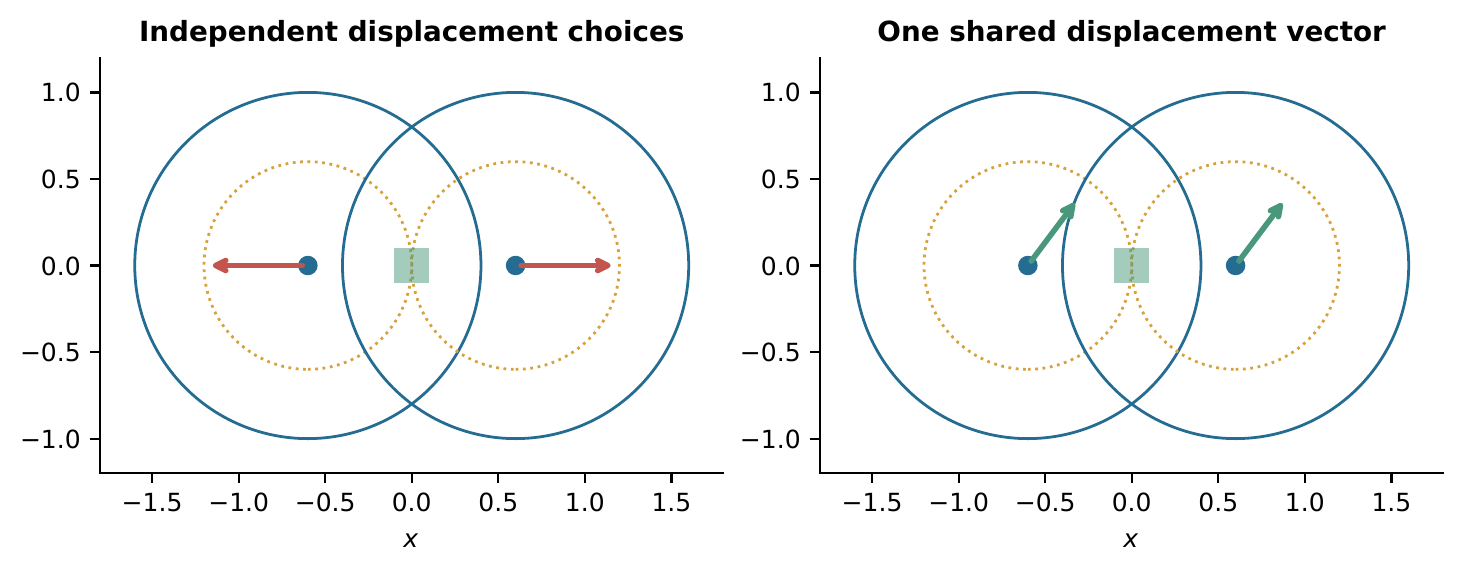
\includegraphics[width=\textwidth]{figures/product-errors.png}
\caption{The difference between product and shared geometric errors in the counterexample of \cref{sec:uncertainty}. Independent choices may move both disks outward. A shared displacement cannot make those opposite moves simultaneously.}
\end{figure*}

\begin{figure*}[tb]
\centering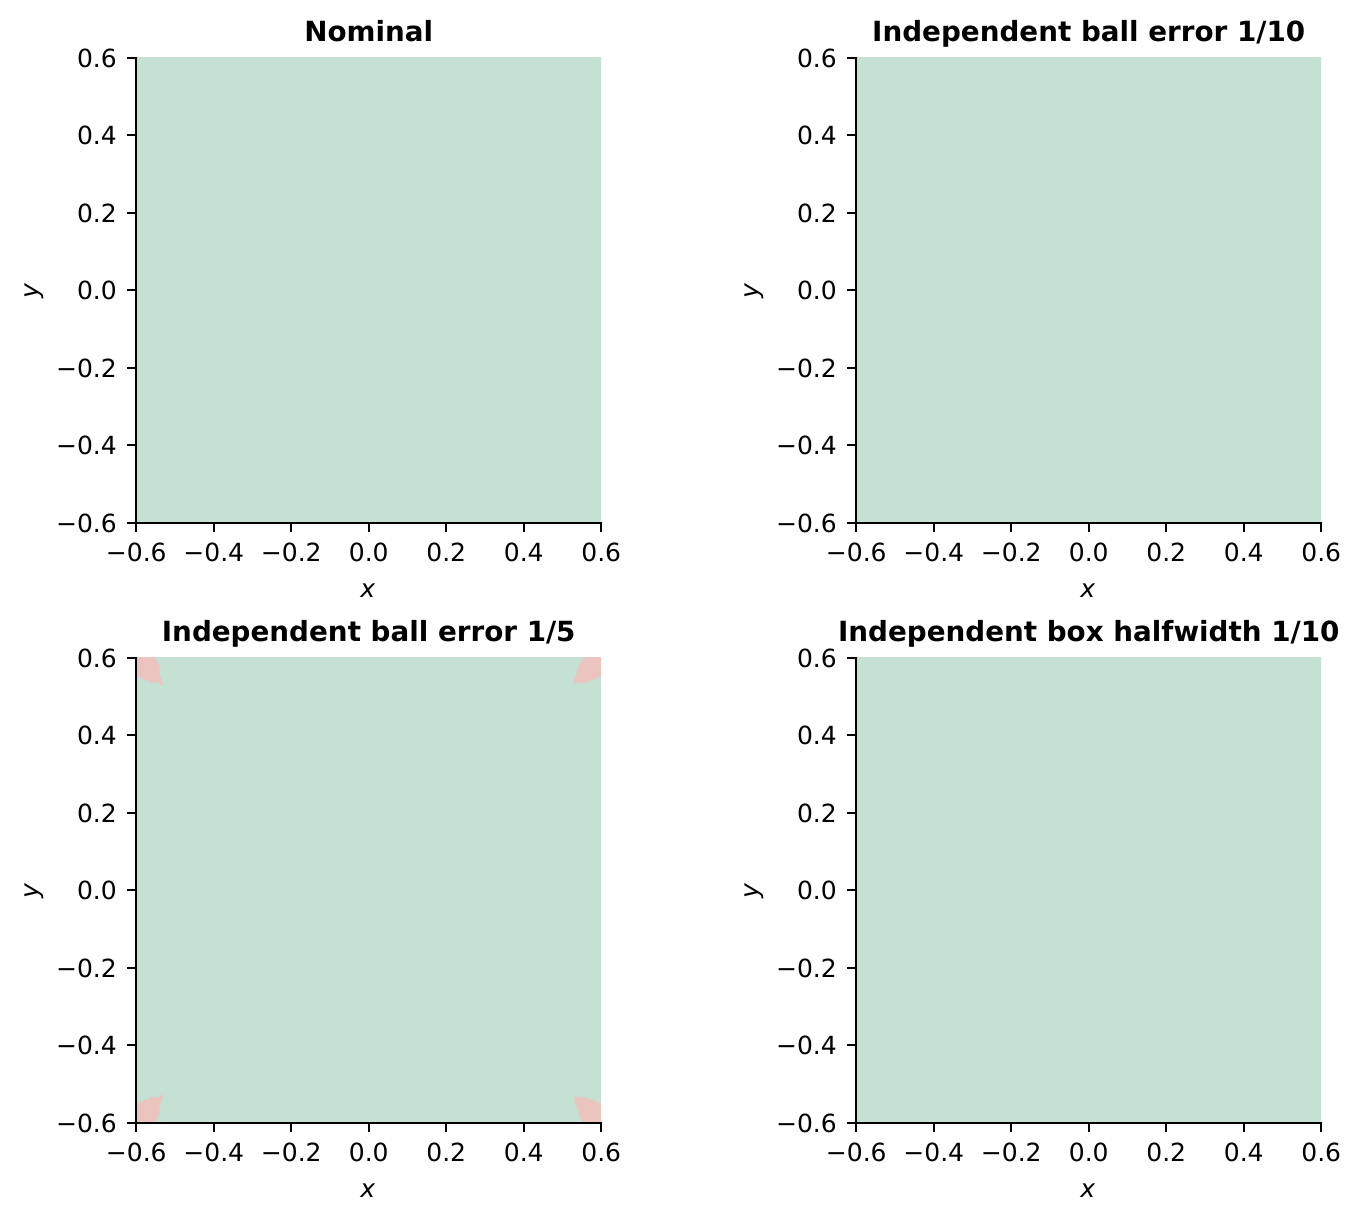
\includegraphics[width=.72\textwidth]{figures/uncertainty-panel.png}
\caption{Guaranteed two-contact target coverage under four placement models. Shading illustrates the winning region; exact target antichains and the support-radius certificate determine acceptance. The box model is represented by finite conjunction bundles, not by an unproved circular approximation.}
\end{figure*}


\section{The resilience polyhedron and certified protection design}
\label{sec:optimization}
The target antichain converts a continuum of spatial failure opportunities into a finite family of cuts. We now use that family to design a protection allocation. The cost model is explicit: allocating a nonnegative value $c_i$ makes deletion of contact $i$ cost $c_i$ to the adversary, and providing that protection consumes $d_i c_i$ units of resource, where $d_i>0$.\footnote{A linear hardening law is a mathematical engineering model. A physical deployment needs an experimentally justified map from protection resource to attack or failure cost. The paper does not infer that law from sensor geometry.}

\subsection{Concavity and weakest-point certificates}
Equation \cref{eq:kappa} shows that $\kappa_T$ is a finite minimum of linear forms. It is concave, positively homogeneous and coordinatewise nondecreasing on $\R_{\ge0}^n$. A minimizing cut $A$ supplies both an attack and a supergradient:
\begin{equation}\label{eq:supergradient}
\kappa_T(c')\le\kappa_T(c)+\boldsymbol1_A\cdot(c'-c).
\end{equation}
Indeed, the right side is $c'(A)$, one of the values over which $\kappa_T(c')$ takes its minimum. At a tie, any convex combination of the tied cut vectors is also a supergradient. The geometric witness associated with the chosen cut identifies where that adversarial value is attained.

Define the fractional blocking polyhedron
\begin{equation}\label{eq:blocking-polyhedron}
\mathcal B_T=\{z\in\R_{\ge0}^n:z(A)\ge1\text{ for every }A\in\mathcal A_T\}.
\end{equation}
For $\tau>0$, the condition $\kappa_T(c)\ge\tau$ is equivalent to $c/\tau\in\mathcal B_T$. This is the standard fractional transversal formulation of a cut hypergraph, here with exact geometric witnesses on the constraints.

\subsection{Primal and dual protection programs}
For a total protection budget $C\ge0$, the best guaranteed deletion cost is
\begin{equation}\label{eq:primal-protection}
\begin{aligned}
V_T(C,d)=\max\ &t\\
\text{subject to }&t\le\sum_{i\in A}c_i\quad(A\in\mathcal A_T),\\
&\sum_i d_i c_i\le C,\qquad c_i\ge0.
\end{aligned}
\end{equation}
The number of cut constraints is bounded quadratically in the geometric input size. This does not make all sensor-placement or wiring problems linear programs: positions and domain assignments remain separate variables in different models.

\begin{theorem}[Protection duality and exact certificates]\label{thm:protection}
The value of \cref{eq:primal-protection} is
\begin{equation}\label{eq:dual-protection}
V_T(C,d)=C\min_{\lambda\in\Delta(\mathcal A_T)}
\max_i\frac{\sum_{A\ni i}\lambda_A}{d_i},
\end{equation}
where $\Delta$ is the probability simplex on the antichain. In particular, if $c\ge0$, $d\cdot c\le C$, $\lambda_A\ge0$, $\sum_A\lambda_A=1$ and
\begin{equation}\label{eq:dual-feasible}
\sum_{A\ni i}\lambda_A\le\mu d_i\quad\text{for every }i,
\end{equation}
then
\begin{equation}\label{eq:certificate-interval}
\min_A c(A)\le V_T(C,d)\le C\mu.
\end{equation}
If the two displayed bounds are equal, these data constitute an exact optimality certificate.
\end{theorem}
\begin{proof}
For any primal-feasible allocation and any dual-feasible pair,
\[
\min_A c(A)\le\sum_A\lambda_Ac(A)
=\sum_i c_i\sum_{A\ni i}\lambda_A
\le\mu\sum_i d_i c_i\le C\mu.
\]
This proves weak duality and the certificate assertion using only finite sums and inequalities.

For equality of the optimal values, assume $C>0$ and put $x_i=d_i c_i/C$. Unused budget can be assigned to any coordinate without decreasing any cut sum, so $x$ can be restricted to the simplex. The normalized value becomes
\[
\max_{x\in\Delta_n}\min_{A\in\mathcal A_T}
\sum_{i\in A}\frac{x_i}{d_i}.
\]
The finite minimax lemma proved in \cref{app:minimax} exchanges this maximum and minimum after the adversary randomizes over cuts. The inner maximum over $x$ is the largest coordinate $\sum_{A\ni i}\lambda_A/d_i$, giving \cref{eq:dual-protection}. For $C=0$, both sides are zero. The feasible sets are compact after normalization, so optima are attained.
\end{proof}

The dual vector is a distribution over weakest target patterns, not a model of the actual failure distribution. Its purpose is to prove that no allocation under the stated resource budget can exceed the certified value. The coordinates $\lambda_A$ can be rational when the input is rational, and equality in \cref{eq:certificate-interval} is then checkable by integer arithmetic.

\begin{corollary}[Fractional transversal interpretation]
If $\varnothing\notin\mathcal A_T$, let
\[
\tau_T^*(d)=\min\{d\cdot z:z\in\mathcal B_T\}.
\]
Then $V_T(C,d)=C/\tau_T^*(d)$. If the antichain contains the empty cut, $V_T=0$.
\end{corollary}
\begin{proof}
For a desired value $t>0$, scaling \cref{eq:blocking-polyhedron} shows that the least resource cost is $t\tau_T^*(d)$. Solving $t\tau_T^*(d)\le C$ gives the formula. If the empty cut occurs, every allocation has $c(\varnothing)=0$.
\end{proof}

\subsection{Duplicating contacts and a sharp budget distinction}
Suppose each original contact $i$ is replaced by $b_i\ge1$ independently labeled copies with exactly the same footprint. Each target cut is expanded by replacing $i$ with all its copies. Under unit deletion costs this can increase the number of required deletions substantially. Under a fixed linear protection budget it has a different effect.

\begin{proposition}[Duplication invariance for the stated protection model]\label{prop:duplication}
If every copy of contact $i$ has the same unit protection coefficient $d_i$ as the original, duplication leaves $V_T(C,d)$ unchanged after aggregating copy allocations. This statement concerns the adversarial linear-cost model, not independent failure probabilities.
\end{proposition}
\begin{proof}
Given copy allocations $c_{i,j}$, put $\bar c_i=\sum_jc_{i,j}$. Every expanded cut has cost $\sum_{i\in A}\bar c_i$, and the budget is $\sum_i d_i\bar c_i$. Thus every copy allocation has exactly the value of a feasible original allocation. Conversely every original allocation is realized by putting its entire $c_i$ on one copy and zero on the remaining copies. Both optimization problems have the same feasible aggregate values.
\end{proof}

The four-corner panel and its duplicated eight-contact version illustrate the distinction. Their minimum numbers of individual deletions are two and four, respectively, but their unit-budget optimal protection values are both $1/2$. Independent Bernoulli reliability can still improve after duplication. A design comparison must specify which of these objectives is being optimized.

\subsection{Numerical proposals and rational verification}
The implementation may ask a floating-point LP solver for a candidate allocation and dual multipliers. It then converts proposed rationals, enforces nonnegativity and budget feasibility, normalizes the dual distribution, and sets $\mu$ to the largest exact ratio in \cref{eq:dual-feasible}. It computes both bounds of \cref{eq:certificate-interval} using rational arithmetic.

Only exact equality establishes verified optimality. If rational recovery yields a gap, the valid conclusion is the interval in \cref{eq:certificate-interval}. Solver status alone is never a proof. The allocations in the analytical examples below are derived symbolically with matching dual bounds, so their optimality does not depend on a numerical optimizer.

\begin{figure}[!htbp]
\centering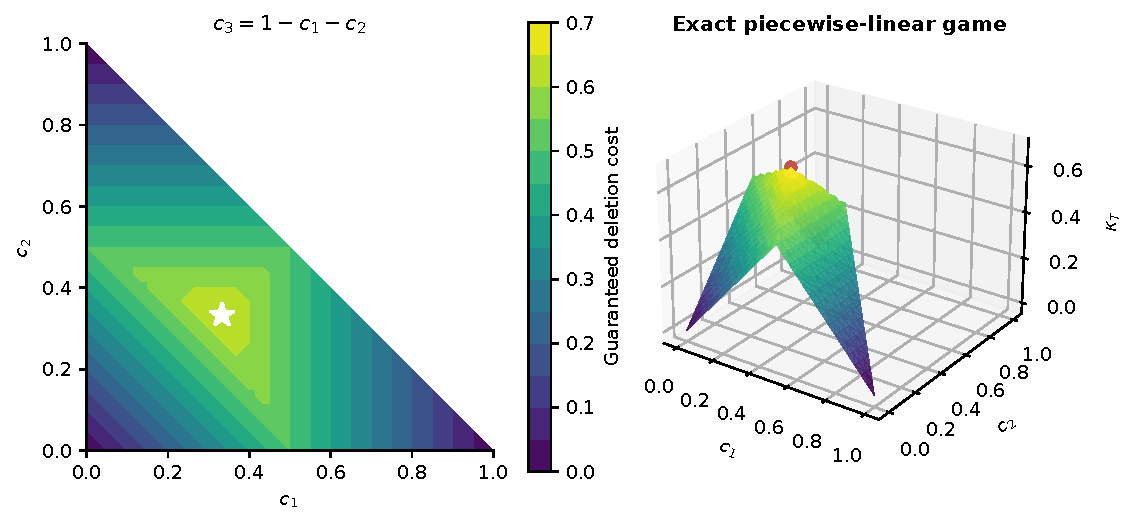
\includegraphics[width=\textwidth]{figures/budget-game.pdf}
\caption{Protection design for the three-asset example. On the unit simplex, $\kappa_T(c)=1-\max_i c_i$. The surface is piecewise linear and attains $2/3$ at the balanced allocation. The diagram displays the exact formula; numerical plotting does not determine the optimum.}
\end{figure}

\FloatBarrier

\section{Fault-domain synthesis and probabilistic reliability}
\label{sec:reliability}
The same geometric certificate supports two different questions: whether every allowed failure is tolerated, and how often a target remains covered under a specified probability law. The first is adversarial and distribution-free. The second requires an actual distribution. Their numerical answers need not agree.

\subsection{Wiring as a hypergraph coloring problem}
Assign contact $i$ to a domain $g(i)\in\{1,\ldots,s\}$. A loss of a domain deletes all contacts assigned to it. For $A\in\mathcal A_T$, write $g(A)=\{g(i):i\in A\}$.

\begin{theorem}[Exact domain-design constraints]\label{thm:domain-design}
A domain assignment survives every loss of at most $q$ complete domains if and only if
\begin{equation}\label{eq:domain-design}
|g(A)|\ge q+1\quad\text{for every }A\in\mathcal A_T.
\end{equation}
The constraints are complete for the continuous target. If an assignment violates one, deleting its at most $q$ represented domains uncovers the associated witness point.
\end{theorem}
\begin{proof}
Apply \cref{thm:relabel} to the domain map. A domain contact set survives every loss of $q$ domains exactly when it has at least $q+1$ members, as in \cref{ex:domains}. \Cref{thm:universal} gives the equivalence and its failure witness.
\end{proof}

For $q=1$, the cut hypergraph must have no monochromatic edge. When all critical cuts have size two, this is ordinary proper graph coloring. Requiring every cut to contain every one of a specified set of colors is the familiar polychromatic or cover-decomposition formulation~\cite{polychromatic}. Equation \cref{eq:domain-design} allows more domains than the number of required surviving alternatives.

The finite constraints can be written as an integer program. Let $z_{ig}$ indicate assignment of contact $i$ to group $g$, and let $u_{Ag}$ indicate whether group $g$ occurs in cut $A$. Require
\[
\sum_g z_{ig}=1,\quad
u_{Ag}\ge z_{ig}\ (i\in A),\quad
u_{Ag}\le\sum_{i\in A}z_{ig},\quad
\sum_g u_{Ag}\ge q+1,
\]
with binary variables. The middle two constraints enforce the exact logical disjunction. A solver-proposed assignment can be checked directly against every certified cut; solver success alone is unnecessary for that verification. Proving that fewer groups are impossible requires a separate lower bound or exhaustive proof.

\begin{example}[An odd-cycle obstruction]\label{ex:oddcycle}
The three-asset geometry in \cref{sec:engineering} has critical patterns $\{1,2\},\{1,3\},\{2,3\}$. It is two-fold covered, but two domains cannot make every pair nonmonochromatic. Three domains suffice. Thus two-fold geometric coverage need not decompose into two separately covering domain layers. This is a finite example of the distinction studied in cover-decomposition theory, not a new general obstruction theorem.
\end{example}

\subsection{Ordinary target-coverage reliability}
Let $F$ now be a random failed-contact set. For ordinary coverage after that failure,
\begin{equation}\label{eq:random-success}
\mathbf1\{T\text{ remains covered}\}
=\prod_{A\in\mathcal A_T}\mathbf1\{A\not\subseteq F\}.
\end{equation}
The analogous formula for domain failures uses the mapped domain antichain. This is the standard minimal-cut representation of a semicoherent reliability system~\cite{barlow}. Some contacts may be irrelevant to the target; relevance of every component is not assumed.

If contacts fail independently with probabilities $p_i$, direct state enumeration gives
\begin{equation}\label{eq:reliability-enumeration}
\mathsf R(p)=\sum_{F\subseteq[n]}\left[\prod_{A\in\mathcal A_T}\mathbf1\{A\not\subseteq F\}\right]
\prod_{i\in F}p_i\prod_{i\notin F}(1-p_i).
\end{equation}
For cuts $A_1,\ldots,A_m$, inclusion--exclusion also gives
\begin{equation}\label{eq:reliability-ie}
\mathsf R(p)=\sum_{J\subseteq[m]}(-1)^{|J|}
\prod_{i\in\bigcup_{j\in J}A_j}p_i.
\end{equation}
The empty $J$ contributes one. Both formulas are exact and generally exponential; the geometric size bound does not turn arbitrary reliability evaluation into a polynomial-time algorithm.\footnote{A polynomial list of minimal cuts can still encode a difficult counting problem. The displayed three-contact calculation is a symbolic evaluation of four successful states, not an asymptotic algorithmic claim.}

For the odd-cycle example with identical independent failure probability $p$,
\[
\mathsf R(p)=(1-p)^3+3p(1-p)^2=1-3p^2+2p^3.
\]
The first equality enumerates the four mutually exclusive successful states, and its polynomial expansion gives the second equality directly.

\subsection{The same four sensors with two wiring choices}
For the four-corner panel, column wiring gives domain cuts $\{1\}$ and $\{2\}$: both domains must work. Diagonal wiring gives the single domain cut $\{1,2\}$: at least one domain must work. Under independent identical domain failure probability $p$,
\begin{equation}\label{eq:wiring-probability}
\mathsf R_{\mathrm{column}}=(1-p)^2,
\qquad
\mathsf R_{\mathrm{diagonal}}=1-p^2.
\end{equation}
At $p=1/10$ these are $81/100$ and $99/100$. The independent-failure law is a chosen model for this comparison. If the two domain failures are arbitrarily dependent but keep the same marginals $p$, the sharp two-event bounds are
\begin{align}
\max(0,1-2p)&\le\mathsf R_{\mathrm{column}}\le1-p,\label{eq:column-frechet}\\
1-p&\le\mathsf R_{\mathrm{diagonal}}\le\min(1,2-2p).\label{eq:diagonal-frechet}
\end{align}
They follow by writing the joint failure probability $a$ between $\max(0,2p-1)$ and $p$. Column success is $1-2p+a$, while diagonal success is $1-a$. At $p=1/10$, the intervals are $[4/5,9/10]$ and $[9/10,1]$.

The diagonal success event contains the column success event for every fixed domain-failure state. Thus its dominance under the same joint distribution does not require independence, even though the numerical values in \cref{eq:wiring-probability} do.

\subsection{Marginal-only reliability as a finite probability program}
If only marginal probabilities and selected dependence constraints are known, introduce a probability $\pi_F$ for each failure state. The sharp lower and upper coverage probabilities solve
\[
\min\text{ or }\max\quad\sum_F \pi_F\,\mathbf1\{A\not\subseteq F\text{ for all }A\in\mathcal A_T\}
\]
subject to $\pi_F\ge0$, $\sum_F\pi_F=1$, $\sum_{F\ni i}\pi_F=p_i$ and any stated additional linear probability constraints. This is the logical probability formulation of Hailperin~\cite{hailperin}, applied to the exact geometric cut list. It can have $2^n$ variables. No efficient solution for every dependence model is claimed.

\subsection{Maintaining a stronger residual requirement}
Equations \cref{eq:random-success,eq:kappa} concern ordinary coverage after a failure. If the desired residual rule is a different monotone predicate $w_0$, the exact condition is instead
\[
w_0(A\setminus F)=1\quad\text{for every }A\in\mathcal A_T.
\]
For nonnegative deletion costs, the exact attack cost becomes
\begin{equation}\label{eq:general-attack}
\min_{A\in\mathcal A_T}\ \min_{B\subseteq A:\,w_0(A\setminus B)=0}c(B).
\end{equation}
If some $A$ already loses under $w_0$, the inner minimum includes $B=\varnothing$ and the value is zero. Otherwise, a failure of an actual active set also fails a contained minimal active set, giving a no-more-expensive cut in that set; conversely that minimal set is realized at its witness. This proves \cref{eq:general-attack}.

For residual $k$-coverage at a pattern of size $a\ge k$, delete its $a-k+1$ cheapest contacts. A general $w_0$ may require a difficult inner optimization, and its complete minimal attack family can be much larger than $\mathcal A_T$. The universal geometric reduction remains exact without implying that every logical optimization is easy.

\begin{figure}[!htbp]
\centering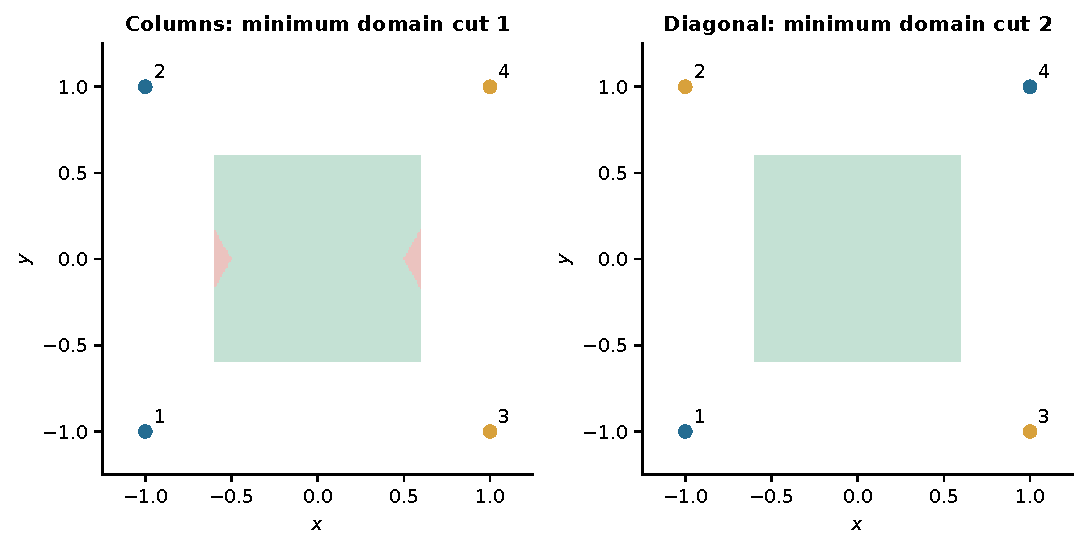
\includegraphics[width=\textwidth]{figures/wiring-comparison.pdf}
\caption{Wiring choices with the same geometry. The target shading illustrates whether two distinct domains are present. Exact certification gives the indicated minimum domain cuts. The geometric and stochastic conclusions use the separately stated models.}
\end{figure}

\begin{figure}[!htbp]
\centering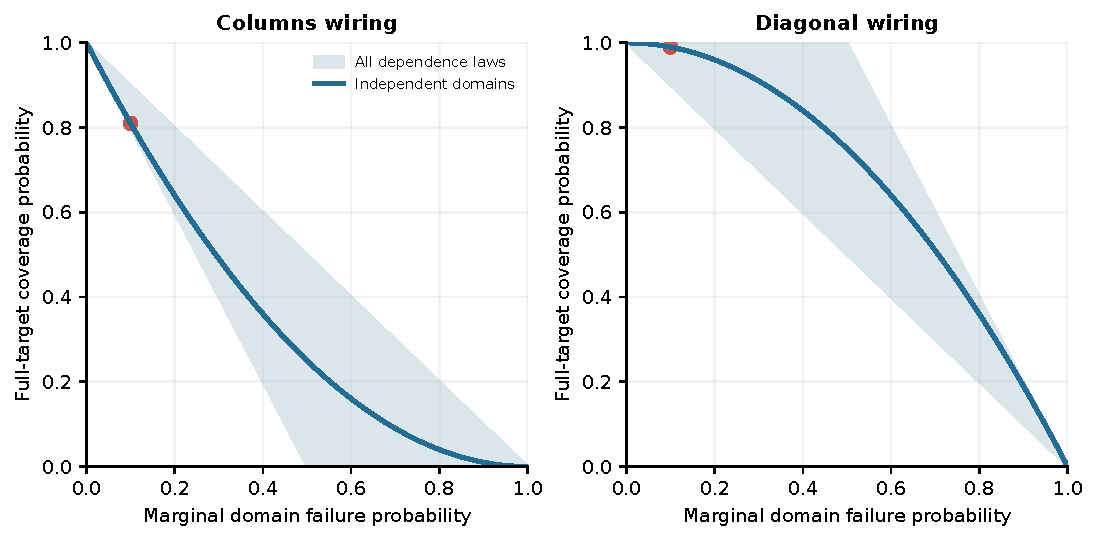
\includegraphics[width=\textwidth]{figures/reliability-curves.pdf}
\caption{Independent-domain reliability and sharp marginal-only bounds for the two wiring choices. The curves are the exact polynomials in \cref{eq:wiring-probability}; the shaded intervals allow arbitrary dependence with fixed marginals.}
\end{figure}

\FloatBarrier

\section{The facet-intersection model}
\label{sec:duality}
Let $N$ be the nerve of a finite family of nonempty compact convex sets. Every face lies in a maximal face. Empty footprints can be removed beforehand without changing any pointwise active set on the remaining labels. Keep the failure rule restricted to those labels.

\begin{definition}
The \emph{winning-face complex} $\Gamma_{\F}(N)$ has one vertex for each $\sigma\in\cP_{\F}$. A nonempty collection $A$ of its vertices is a simplex if
\begin{equation}\label{eq:Gamma}
\bigcup_{\sigma\in A}\sigma\in N.
\end{equation}
With $\M=\Max N$, the \emph{facet-intersection complex} has nonempty faces
\begin{equation}\label{eq:dual-intro}
\cC_{\F}(N)=\{B\subseteq\M:B\ne\varnothing,\ \bigcap_{M\in B}M\notin\F\}.
\end{equation}
\end{definition}
Upward closure of winning sets implies that \cref{eq:dual-intro} is closed under taking nonempty subsets of $A$: removing a maximal face makes the intersection larger. Thus it does define an abstract simplicial complex. In contrast, enlarging a contact set in $N$ need not preserve being a face, so the directions of the union and intersection tests must not be reversed.

\begin{theorem}[Coverage duality]\label{thm:duality}
For compact convex footprints and any failure family,
\begin{equation}\label{eq:homotopy-chain}
R_{\F}\simeq\abs{\Gamma_{\F}(N)}\simeq\abs{\cC_{\F}(N)}.
\end{equation}
The combinatorial equivalence is an instance of Dowker duality~\cite{dowker,chowdhury} for the containment relation between winning faces and maximal nerve faces. It does not require a bound on the sizes of those faces.
\end{theorem}
\begin{proof}
By \cref{prop:pointwise}, the sets $D_\sigma$, indexed by $\sigma\in\cP_{\F}$, cover $R_{\F}$. A finite intersection of these sets is
\[
\bigcap_{\sigma\in A}D_\sigma=D_{\bigcup_{\sigma\in A}\sigma}.
\]
It is nonempty exactly when \cref{eq:Gamma} holds, and when nonempty it is compact and convex. The finite closed-convex nerve theorem therefore identifies its nerve $\Gamma_{\F}(N)$ with $R_{\F}$ up to homotopy. The closed-convex hypothesis is used here; an arbitrary cover by closed contractible sets would not justify the same argument~\cite{bauer}.

For completeness, we prove the combinatorial equivalence by explicit maps. Let $Q_\Gamma$ and $Q_C$ be the nonempty face posets of $\Gamma_{\F}(N)$ and $\cC_{\F}(N)$. Set
\begin{align}
f(A)&=\left\{M\in\M:\bigcup_{\sigma\in A}\sigma\subseteq M\right\},\label{eq:f-map}\\
g(B)&=\left\{\sigma\in\cP_{\F}:\sigma\subseteq\bigcap_{M\in B}M\right\}.\label{eq:g-map}
\end{align}
For a face $A$, its union is in $N$, so $f(A)$ is nonempty. The intersection of all members of $f(A)$ contains that union, which contains a winning face. Hence $f(A)$ is a face of $\cC_{\F}$. For a face $B$, its intersection $I_B$ is a winning face of $N$. In particular, $I_B\in g(B)$, and the union of all members of $g(B)$ is exactly $I_B$. Thus $g(B)$ is a nonempty face of $\Gamma_{\F}$.

Both maps reverse inclusion. Their composites preserve inclusion and satisfy
\begin{equation}\label{eq:closure-inequalities}
A\subseteq g f(A),\qquad B\subseteq f g(B).
\end{equation}
For the first inclusion, each $\sigma\in A$ lies in every maximal face containing the union of $A$. For the second, $\bigcup g(B)=I_B$ lies in every $M\in B$.

An order-preserving map pointwise above the identity induces a map homotopic to the identity on the order complex; a proof by prisms is given in \cref{app:posets}. An order-reversing map also induces a simplicial map on order complexes, by reversing the order of each image chain. Applying this observation to \cref{eq:closure-inequalities}, the realizations of $f$ and $g$ are mutually inverse up to homotopy. The order complexes are the barycentric subdivisions of $\Gamma_{\F}$ and $\cC_{\F}$, whose realizations are homeomorphic to those of the original complexes.

If there is no winning nerve face, all three spaces are empty by definition and the assertion is immediate.
\end{proof}

\begin{corollary}[Minimal-coalition shadow]\label{cor:minimal}
Let $\Lambda_{\F}=\Min\W\cap N$. Form a complex on $\Lambda_{\F}$ by declaring $A$ a face when $\bigcup_{\sigma\in A}\sigma\in N$. Its realization is homotopy equivalent to $R_{\F}$ and to $\abs{\cC_{\F}(N)}$. For $\F=\F_{k-1}$ this is exactly the $k$-shadow $\Delta_k(N)$.
\end{corollary}
\begin{proof}
The subfamily $(D_\sigma)_{\sigma\in\Lambda_{\F}}$ is still a finite convex cover of $R_{\F}$ by \cref{eq:region-unions}. Its nerve is the stated union complex. Apply the same closed-convex nerve theorem and \cref{thm:duality}.
\end{proof}

Using every winning face in $\Gamma_{\F}$ is convenient for naturality but unnecessary in computation. Using only minimal winners is often still expensive. The dual complex evaluates the predicate only on intersections of maximal nerve faces and does not list either collection of coalitions.

\begin{theorem}[Increasing failure families]\label{thm:natural}
Fix the footprints, their nerve $N$ and its full set of maximal faces $\M$. If $\F_1\subseteq\F_2$, there are inclusions
\[
\Gamma_{\F_2}\subseteq\Gamma_{\F_1},\qquad
\cC_{\F_2}\subseteq\cC_{\F_1},\qquad
R_{\F_2}\subseteq R_{\F_1}.
\]
For every homological degree and fixed coefficient field the isomorphisms in \cref{thm:duality} can be taken natural for these inclusions. Therefore a nested sequence of failure families gives isomorphic homology persistence modules in the geometric and dual models.
\end{theorem}
\begin{proof}
A face winning against $\F_2$ wins against $\F_1$, proving the first two inclusions directly from their defining tests. The region inclusion is \cref{lem:monotonicity}. On nonempty face posets the map $f$ in \cref{eq:f-map} is independent of the failure family: it lists all maximal faces containing a given union. Hence its square with the two inclusion maps commutes exactly. Since $f$ is an objectwise homotopy equivalence, it induces a natural homology isomorphism.

The convex cover for $\F_2$ is a subfamily of the one for $\F_1$, with the same geometric set attached to each surviving index. The functorial closed-convex nerve theorem supplies natural homology isomorphisms for this inclusion. In the disk setting, compatible semialgebraic triangulations and the double-chain comparison in \cref{app:nerve} give an additional chain-level explanation. Composing the two comparisons proves the assertion.
\end{proof}

\begin{remark}[Changing geometry]
Maximal nerve faces can change when radii or positions change. The literal vertex sets of the corresponding facet-intersection complexes then need not be nested. \Cref{thm:natural} fixes the geometry; it does not assert a raw simplicial inclusion for moving radii. Geometric perturbation inclusions are proved in \cref{sec:certificates}, and standard multicover bifiltrations already address simultaneous radius and multiplicity parameters~\cite{corbet,alonso}.
\end{remark}

\begin{proposition}[Two-skeleton sufficiency]\label{prop:two-skeleton}
For any finite complex $K$, its full two-skeleton determines $H_0(K;\FF)$ and $H_1(K;\FF)$. If its graph has $V$ vertices, $E$ edges and $c$ components, then
\begin{equation}\label{eq:betti-formula}
b_0=c,\qquad b_1=E-V+c-\rank\partial_2.
\end{equation}
\end{proposition}
\begin{proof}
The chain groups and boundary maps relevant to degrees zero and one are
\[
C_2(K;\FF)\xrightarrow{\partial_2}C_1(K;\FF)\xrightarrow{\partial_1}C_0(K;\FF).
\]
Higher-dimensional simplices do not change these maps. In the graph of $K$, the incidence matrix has rank $V-c$: a spanning tree gives rank $v-1$ on a connected component with $v$ vertices, and every additional edge has boundary equal to the sum of boundaries along its tree path. Thus $\dim\ker\partial_1=E-V+c$. Quotient by $\im\partial_2$ to obtain \cref{eq:betti-formula}.
\end{proof}

\begin{example}[The dual complex need not be a flag complex]
Take maximal nerve faces $M_1=\{1,2\}$, $M_2=\{2,3\}$ and $M_3=\{1,3\}$, with the rule that one contact suffices. Every pair of maximal faces intersects in a winning singleton, but all three have empty intersection. The dual complex has three edges and no triangle. Filling its graph clique would erase its first homology. So the three-fold facet intersection must be checked for every candidate triangle.
\end{example}

\section{Exact geometry without nerve-face enumeration}
\label{sec:geometry}
The duality theorem is useful only if the maximal nerve faces can be obtained reliably. For disks, a finite arrangement construction avoids listing every intersecting subfamily. In this section
\[
D_i=\{x\in\R^2:\|x-c_i\|\le r_i\},\qquad r_i\ge0,
\]
and coincident disks keep their distinct contact labels.

\begin{definition}
The \emph{witness list} consists of the leftmost point $\ell_i=(c_{i,x}-r_i,c_{i,y})$ of each disk and all intersections of the boundaries of pairs of disks whose supporting circles are distinct. A zero-radius disk contributes its center through $\ell_i$. A coincident pair contributes no additional points. The label of a witness $x$ is $L(x)=\{i:x\in D_i\}$.
\end{definition}

\begin{theorem}[Quadratic witness bound]\label{thm:witness}
Every maximal face of the nerve is the label of a point on the witness list. Hence the inclusion-maximal nonempty witness labels are exactly $\Max N$, and
\begin{equation}\label{eq:witness-count}
\abs{\Max N}\le n+2\binom n2=n^2.
\end{equation}
The assertion allows unequal radii, tangency, zero radii and coincident disks.
\end{theorem}
\begin{proof}
Every witness label is a nerve face, because the witness itself lies in all its labeled disks. Let $\sigma$ be a maximal nerve face and set $K=\bigcap_{i\in\sigma}D_i$. This is nonempty and compact. Choose a point $x\in K$ with minimal first coordinate.

If $\sigma$ contains a zero-radius disk, then $K$ consists of its center, which is a listed witness. Suppose all its disks have positive radius. At least one constraint is active at $x$: if all were strict, a small open neighborhood of $x$ would lie in $K$, contradicting minimality. If two active constraints have distinct supporting circles, $x$ is one of their boundary intersections and is listed.

The remaining case has only one distinct active supporting circle, possibly repeated with several labels. Every other disk of $\sigma$ contains a neighborhood of $x$. In a sufficiently small neighborhood the only effective constraint is therefore the closed disk bounded by that active circle. Unless $x$ is its leftmost point, there are points of that disk arbitrarily close to $x$ with smaller first coordinate. They still satisfy every locally slack constraint, a contradiction. Thus $x$ is the leftmost point of an active disk and is listed.

In all cases $\sigma\subseteq L(x)$. The label is a nerve face and $\sigma$ is maximal, so equality follows. Taking maximal labels removes only proper subfaces and duplicates. Each noncoincident pair of circles has at most two intersection points, which proves \cref{eq:witness-count}.
\end{proof}

\begin{remark}
The extremal-point argument is an elementary disk-arrangement method. The bound concerns the number of maximal nerve faces, not the number of all nerve faces or all simplices of the dual complex. A single maximal face on $n$ labels contains $2^n-1$ nonempty nerve faces. Likewise $n^2$ dual vertices alone do not give a quadratic bound on all dual simplices.
\end{remark}

\subsection{Circle intersections in a quadratic extension}
The witness labels can be determined without evaluating square roots approximately. Suppose $c_i\ne c_j$ and put
\begin{align}
d&=c_j-c_i,\qquad s=d\cdot d>0,\nonumber\\
\alpha&=\frac{s+r_i^2-r_j^2}{2s},\qquad
h=\frac{r_i^2}{s}-\alpha^2,\label{eq:circle-parameters}\\
B&=c_i+\alpha d,\qquad P=(-d_y,d_x).\nonumber
\end{align}
If $h<0$, the boundaries do not meet. If $h=0$, they meet at $B$. If $h>0$, their intersections are
\begin{equation}\label{eq:circle-points}
x_{\pm}=B\pm\sqrt h\,P.
\end{equation}
Indeed, subtracting the two circle equations gives the line $(x-c_i)\cdot d=\alpha s$. Substituting $x=B+tP$ in the first equation gives $t^2=h$. This also covers internal and external tangency.

For a third disk, write $z=B-c_k$. Membership of $x_\pm$ is the inequality
\begin{equation}\label{eq:quadratic-membership}
A+C\sqrt h\le0,
\quad A=z\cdot z+h(P\cdot P)-r_k^2,
\quad C=\pm2z\cdot P.
\end{equation}
When input numbers are rational, $A,C,h$ are rational. No coordinates of a square-root point need be rounded.

\begin{lemma}[Exact radical sign]\label{lem:sign}
Let $A,C,h\in\mathbb Q$ with $h\ge0$. The truth of $A+C\sqrt h\le0$ is determined by rational comparisons as follows:
\begin{enumerate}
\item if $h=0$ or $C=0$, test $A\le0$;
\item if $A=0$ and $h>0$, test $C\le0$;
\item if $A<0$ and $C<0$, the inequality holds; if $A>0$ and $C>0$, it fails;
\item if $A>0$ and $C<0$, test $A^2\le C^2h$;
\item if $A<0$ and $C>0$, test $C^2h\le A^2$.
\end{enumerate}
\end{lemma}
\begin{proof}
The first three cases follow from signs. In the fourth case the desired inequality is $A\le(-C)\sqrt h$, with both sides nonnegative, so squaring preserves its direction and equivalence. In the fifth case it is $C\sqrt h\le -A$, again with nonnegative sides. These cases exhaust all possibilities. Equality is retained because the disks are closed.
\end{proof}

\subsection{Enumeration and chain construction}
\begin{algorithm}[Exact facet computation]\label{alg:facets}
\leavevmode
\begin{enumerate}
\item Interpret the finite coordinates and radii as rationals; reject negative radii or nonfinite input.
\item Label the $n$ leftmost points by squared-distance comparisons.
\item For each pair of distinct centers, compute \cref{eq:circle-parameters}. If $h\ge0$, label its one or two boundary intersections using \cref{lem:sign}. Pairs with equal centers require no boundary computation.
\item Delete empty labels and duplicates. Sort the remaining masks by decreasing cardinality, and retain a mask exactly when it is not contained in a previously retained mask.
\end{enumerate}
The output is $\Max N$ by \cref{thm:witness}.
\end{algorithm}

With $m=\abs\M$ and a winning predicate $w$, the full dual two-skeleton is constructed as follows. Retain $M\in\M$ as a vertex if $w(M)$ is true. An edge $\{M_i,M_j\}$ is retained if $w(M_i\cap M_j)$ is true. A candidate triangle is retained if all three edges exist and $w(M_i\cap M_j\cap M_k)$ is true. The edge checks are redundant mathematically for an upward-closed rule, but they avoid unnecessary work and ensure a consistent boundary indexing.

Each triangle gives a boundary column with three nonzero edge entries over $\FF$. Gaussian elimination determines its rank, while a union--find structure computes the graph components. \Cref{eq:betti-formula} then gives both Betti numbers.

\begin{theorem}[Finite exact low-degree computation]\label{thm:algorithm}
For $n$ closed planar disks with rational input data, and an exactly evaluable monotone winning predicate, \cref{alg:facets} and the complete dual two-skeleton compute $H_0$ and $H_1$ of the surviving region exactly over $\FF$. Witness labeling uses $O(n^3)$ rational sign tests. A naive maximal-label filter uses $O(n^4)$ mask-containment tests. The dual two-skeleton uses at most $n^2$ vertices, $\binom{n^2}{2}$ edge predicates and $\binom{n^2}{3}$ triangle predicates.
\end{theorem}
\begin{proof}
There are at most $n^2$ witnesses and $n$ membership tests per witness. A quadratic comparison of at most $n^2$ labels bounds the naive filtering step. Correctness of those steps follows from \cref{thm:witness,lem:sign}. The simplex count follows from $m\le n^2$, and every simplex through dimension two is included by its defining predicate. \Cref{thm:duality,prop:two-skeleton} identify the resulting homology with that of the surviving region.
\end{proof}

This is an arithmetic-operation and oracle-query bound. It is not a unit-time bit-complexity bound: rational numerator sizes, arbitrary-precision mask operations, predicate costs and elimination all matter. The worst-case number of dual triangles is $O(n^6)$, and the full dual complex may have exponentially many simplices. For $H_j$ with fixed $j$, its full $(j+1)$-skeleton suffices, giving at most $O(n^{2j+4})$ simplex tests by the same argument. These bounds are deliberately separate from the much more refined multicover bifiltration algorithms of~\cite{corbet,alonso}.

\subsection{Equal-radius verification by a different geometric formula}
For equal-radius disks there is another exact intersection criterion, expressed through minimum enclosing circles of center triples. If $a,b,c$ are three centers, let
\[
u=\|a-b\|^2,\quad v=\|a-c\|^2,\quad w=\|b-c\|^2,
\quad J=(b-a)_x(c-a)_y-(b-a)_y(c-a)_x.
\]
The squared minimum enclosing radius is
\begin{equation}\label{eq:mec}
\rho^2(a,b,c)=
\begin{cases}
\max(u,v,w)/4,&2\max(u,v,w)\ge u+v+w,\\[2pt]
uvw/(4J^2),&2\max(u,v,w)<u+v+w.
\end{cases}
\end{equation}
The first case includes right, obtuse, collinear and coincident configurations. The second is the circumradius formula for an acute triangle; its denominator is nonzero. Two equal-radius disks meet if their center distance squared is at most $4r^2$, and three meet if and only if $\rho^2\le r^2$. Planar Helly's theorem extends the triple criterion to every larger subfamily.

Equation \cref{eq:mec} supplies a separate analytical criterion for testing a proposed facet and its one-contact extensions. Completeness of the witness list is supplied by \cref{thm:witness}; checking triples alone would not, for an arbitrary list of purported facets, prove that completeness.

\section{Continuous target certificates and perturbation control}
\label{sec:certificates}
A homotopy model describes the surviving region once the footprints are known. An engineering target is additional data: a compact set $T$ for which one wants $T\subseteq R_{\F}$. This section gives a sufficient test for that inclusion, with the same winning rule as the dual complex. The constant in the triangle bound is the familiar planar covering constant used in the companion coverage archive~\cite{ecog}; the extension here is its formulation for a general monotone failure predicate.

\subsection{The winning margin}
Assume that $\W$ is nonempty and define the contact slack functions
\[
g_i(x)=r_i-\|x-c_i\|.
\]
The \emph{winning margin} is
\begin{equation}\label{eq:margin}
\phi_{\F}(x)=\max_{\sigma\in\Min\W}\ \min_{i\in\sigma}g_i(x).
\end{equation}
Minimal winning sets in this formula range over the full contact label set; they need not have a nonempty footprint intersection. The formula describes a real-valued function even outside the covered region. If $\W$ is empty, $R_{\F}$ is empty and target certification is handled separately.

\begin{lemma}[Margin semantics and Lipschitz control]\label{lem:margin}
The function $\phi_{\F}$ is $1$-Lipschitz. For each real $t$,
\begin{equation}\label{eq:slack-winning}
\phi_{\F}(x)\ge t\quad\Longleftrightarrow\quad
\{i:g_i(x)\ge t\}\notin\F.
\end{equation}
In particular,
\begin{equation}\label{eq:margin-region}
R_{\F}=\{x:\phi_{\F}(x)\ge0\}.
\end{equation}
\end{lemma}
\begin{proof}
By the reverse triangle inequality, $\abs{g_i(x)-g_i(y)}\le\|x-y\|$. If finite collections of functions each change by at most $d$ between two points, their minima and their maxima change by at most $d$. Applying this twice to \cref{eq:margin} proves the Lipschitz assertion.

The left side of \cref{eq:slack-winning} means that one minimal winning set has every contact slack at least $t$. This is equivalent to the slack-threshold contact set containing a winning set, and therefore to that set itself being winning. At $t=0$, it is precisely the active contact set of the closed disks; use \cref{prop:pointwise}.
\end{proof}

For ordinary $k$-fold coverage, $\phi_{\F}$ is the $k$th largest slack. For a failure budget, sort the slacks in decreasing order and accumulate failure costs until their sum first exceeds $B$; the corresponding slack is the margin. Ties can be processed as a block, and zero-cost contacts do not change the threshold. For $q$ domain losses, first maximize the slack within each domain and then take the $(q+1)$st largest domain slack. These are ways of evaluating the same finite maximum--minimum formula, not assumptions of statistical independence.

\subsection{A sharp triangle sampling bound}
\begin{lemma}[Distance to triangle vertices]\label{lem:triangle}
Let $T=\conv\{v_1,v_2,v_3\}\subset\R^2$ and $D=\max_{i,j}\|v_i-v_j\|$. Every $x\in T$ satisfies
\begin{equation}\label{eq:triangle-distance}
\min_i\|x-v_i\|\le\frac D{\sqrt3}.
\end{equation}
The constant is sharp for an equilateral triangle.
\end{lemma}
\begin{proof}
If the triangle is degenerate, any point of its segment lies within half the segment length of one of its extreme vertices, so the bound follows. Otherwise partition $T$ into its three clipped vertex Voronoi cells. On a cell, squared distance to its vertex is convex and attains its maximum at an extreme point of that cell. On the boundary of $T$, a point of an edge lies within half the edge length of one of that edge's endpoints, giving a bound $D/2$ for its nearest vertex.

The only possible interior Voronoi vertex is the circumcenter. If it lies inside $T$, the triangle is acute and its largest angle $A$ lies between $\pi/3$ and $\pi/2$. The circumradius is $D/(2\sin A)\le D/\sqrt3$. These are all the possible cell extremes relevant to a maximum, proving the claim. In an equilateral triangle, the center is at distance $D/\sqrt3$ from every vertex, proving sharpness.
\end{proof}

\begin{theorem}[Continuous target certificate]\label{thm:target}
Let a compact target $T$ be the union of finitely many closed planar triangles. For each triangle $\tau$ let $D_\tau$ be its diameter. If every vertex $v$ of every triangle satisfies
\begin{equation}\label{eq:triangle-cert}
\phi_{\F}(v)\ge D_\tau/\sqrt3,
\end{equation}
then $T\subseteq R_{\F}$. The condition is sufficient, and a failed certificate is inconclusive about actual coverage.
\end{theorem}
\begin{proof}
Fix $x\in\tau$ and choose a vertex $v$ at distance at most $D_\tau/\sqrt3$ by \cref{lem:triangle}. By \cref{lem:margin},
\[
\phi_{\F}(x)\ge\phi_{\F}(v)-\|x-v\|\ge0.
\]
Thus $x\in R_{\F}$. Apply the same argument to every triangle.
\end{proof}

The winning coalition is allowed to differ between vertices and triangles. The argument only needs a winning coalition at the selected nearest vertex with enough margin to reach the point. It does not assume that one fixed coalition covers an entire target. For an equilateral triangle with one disk of radius $b<D/\sqrt3$ centered at each vertex, the center is uncovered although each vertex has ordinary one-fold margin $b$. Hence a smaller universal vertex-margin constant cannot replace $1/\sqrt3$ in this form of certificate.

\begin{proposition}[Exact evaluation of a triangle certificate]\label{prop:exact-target}
For rational disk and triangle data, the sufficient test in \cref{thm:target} can be decided using the same radical sign predicate as \cref{lem:sign}. Let $h=D_\tau^2/3$. At a vertex $v$, keep contact $i$ precisely when
\begin{equation}\label{eq:exact-target}
r_i^2\ge h,\qquad
\|v-c_i\|^2-r_i^2-h+2r_i\sqrt h\le0.
\end{equation}
The triangle is certified if and only if the retained set at each vertex wins.
\end{proposition}
\begin{proof}
By \cref{eq:slack-winning}, the desired test is winning of the set with $r_i-\|v-c_i\|\ge\sqrt h$. This requires $r_i\ge\sqrt h$, equivalent to the first inequality because $r_i\ge0$. Subject to it, both sides of $\|v-c_i\|\le r_i-\sqrt h$ are nonnegative. Squaring is therefore reversible and gives the second inequality of \cref{eq:exact-target}. All coefficients outside $\sqrt h$ are rational, so \cref{lem:sign} applies.
\end{proof}

The test \cref{eq:exact-target} includes zero-diameter triangles and zero-radius contacts, and it needs only the three eligible contact masks and the exact squared diameter; no homology computation enters.

\subsection{Uncertain geometry}
Suppose the actual parameters satisfy
\[
\|c_i'-c_i\|\le\epsilon_i,\qquad |r_i'-r_i|\le\eta_i,
\quad r_i,r_i'\ge0,
\]
and put $\delta=\max_i(\epsilon_i+\eta_i)$. Write $\phi$ and $\phi'$ for the two winning margins with the same failure family.

\begin{theorem}[Uniform margin stability]\label{thm:stability}
For all $x$,
\begin{equation}\label{eq:margin-stability}
|\phi(x)-\phi'(x)|\le\delta.
\end{equation}
In particular,
\begin{equation}\label{eq:stable-sandwich}
\{\phi\ge\delta\}\subseteq R_{\F}(D')\subseteq\{\phi\ge-\delta\}.
\end{equation}
If every target triangle vertex obeys
\[
\phi(v)\ge\delta+D_\tau/\sqrt3,
\]
then every geometry satisfying the error bounds covers the entire target under the prescribed failures.
\end{theorem}
\begin{proof}
For every $i$,
\[
|g_i(x)-g_i'(x)|\le |r_i-r_i'|+
\big|\|x-c_i\|-\|x-c_i'\|\big|\le\eta_i+\epsilon_i\le\delta.
\]
Finite minima and maxima preserve this uniform bound, proving \cref{eq:margin-stability}. If $\phi(x)\ge\delta$, then $\phi'(x)\ge0$. If $\phi'(x)\ge0$, then $\phi(x)\ge-\delta$. This proves the inclusions. For a target point choose its nearby triangle vertex and apply both the geometric Lipschitz bound and the parameter error bound.
\end{proof}

For each offset $t$ the same argument gives $\{\phi\ge t+\delta\}\subseteq\{\phi'\ge t\}\subseteq\{\phi\ge t-\delta\}$. Thus the superlevel homology modules are $\delta$-interleaved, with the superlevel parameter ordered in the usual reverse direction. This statement concerns the geometric modules; no unproved nesting of changing maximal-facet vertex sets is required.

\begin{corollary}[A robust homology lower bound]
Let $X^-=\{\phi\ge\delta\}$ and $X^+=\{\phi\ge-\delta\}$. For any admissible actual geometry and any degree $j$,
\[
\dim H_j(R_{\F}(D'))\ \ge\
\rank\bigl(H_j(X^-)\longrightarrow H_j(X^+)\bigr).
\]
\end{corollary}
\begin{proof}
The inclusion-induced map on the right factors through $H_j(R_{\F}(D'))$ by \cref{eq:stable-sandwich}. The rank of a factorization cannot exceed the dimension of its middle vector space.
\end{proof}

The lower bound does not rule out extra classes born and killed inside the uncertainty interval. Equal endpoint Betti numbers, or even an isomorphism between endpoints, need not give the exact Betti number of every intermediate geometry. For a target failure certificate, on the other hand, a point $x\in T$ with $\phi(x)<-\delta$ remains uncovered for every admissible actual geometry by \cref{eq:margin-stability}. These are distinct conclusions and require distinct data.

\section{Analytical design examples}
\label{sec:engineering}
The examples in this section are exact models, not simulations. All thresholds, probabilities and optimization values are derived below or in \cref{app:worked}. The accompanying plots display the formulas and geometry. They do not supply a numerical premise for a proof.

\subsection{Three assets and an obstruction to two-domain protection}
Place contacts at $(-1,0)$, $(1,0)$ and $(0,3/2)$ with common radius $6/5$. Around the three pairwise midpoints $(0,0)$, $(-1/2,3/4)$ and $(1/2,3/4)$, take triangular target patches with offsets
\[
(-1/20,-1/20),\quad(1/20,-1/20),\quad(0,1/20).
\]
Each patch lies in exactly its intended pair of disks; the complete inequalities are given in \cref{app:worked}. Thus
\[
\mathcal A_T=\{\{1,2\},\{1,3\},\{2,3\}\}.
\]
Two contacts always cover every target point, but two domains cannot protect all three patches against a domain loss. If the first two contacts have different colors, the third must differ from both to avoid a monochromatic pair. Three domains are necessary and sufficient. This elementary odd-cycle argument distinguishes overlap count from a decomposition into independently surviving layers.\footnote{The example is a finite illustration of cover-decomposition and polychromatic-coloring questions, which have a substantial prior literature~\cite{polychromatic}. It is not presented as a newly discovered coloring obstruction.}

\begin{figure}[!htbp]
\centering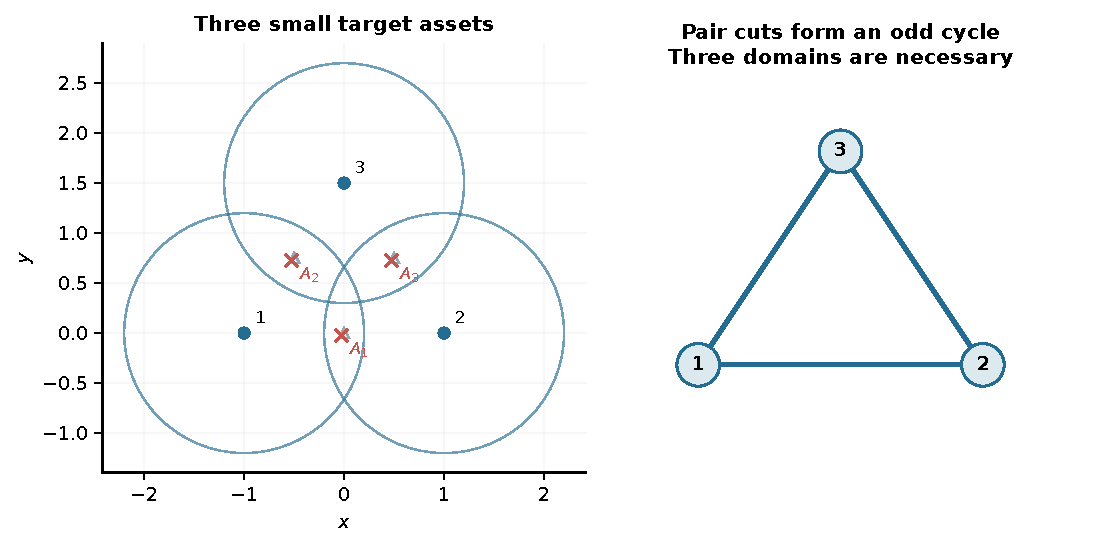
\includegraphics[width=\textwidth]{figures/odd-cycle.pdf}
\caption{The three exact target patches and their critical pair cuts. Each patch can be checked by the rational squared-distance inequalities in the appendix. The cut graph is an odd cycle.}
\end{figure}

Under unit total protection resource and unit protection coefficients, the cut cost is
\[
\kappa_T(c)=\min(c_1+c_2,c_1+c_3,c_2+c_3).
\]
If the full resource is used, this equals $1-\max_i c_i\le2/3$. Equality holds at $c_i=1/3$. Equivalently, a uniform dual distribution on the three cuts gives $\mu=2/3$, proving the exact optimality value through \cref{thm:protection}. For independent contact failure probability $p$, the target survives precisely when at most one contact fails, giving $1-3p^2+2p^3$.
\FloatBarrier

\subsection{A square target with four corner contacts}
Take target $[-a,a]^2$ with $a=3/5$, sites $(\pm1,\pm1)$ and nominal radius $9/5$. Label them in order as $(-1,-1)$, $(-1,1)$, $(1,-1)$ and $(1,1)$. The critical patterns are
\begin{equation}\label{eq:panel-cuts}
\{1,2\},\quad\{1,3\},\quad\{2,4\},\quad\{3,4\}.
\end{equation}
To verify completeness, write $u=\max(|x|,|y|)$ and $v=\min(|x|,|y|)$. The second-nearest squared distance is
\[
2+u^2+v^2-2u+2v,\qquad 0\le v\le u\le a.
\]
This convex quadratic has maximum $2+2a^2=68/25$ at a vertex of the parameter triangle. The two nearest corners share a side; at a tie the active set contains one of those adjacent pairs. Since $81/25>68/25$, every active set contains a listed pair.

The point $(-11/20,0)$ has squared distances $481/400$ to the left corners and $1361/400$ to the right corners. Since $(9/5)^2=1296/400$, its active set is exactly $\{1,2\}$. The three symmetric points realize the other pairs. This proves \cref{eq:panel-cuts} without an enumeration procedure.

\subsection{An exact power--resilience staircase}
For the same geometry, let $t=r^2$ and assign unit deletion costs. The maxima of the first through fourth ordered squared distances are
\[
2,\qquad68/25,\qquad89/25,\qquad128/25.
\]
The formulas for all four distances and their maxima are derived in \cref{app:worked}. Therefore the complete deletion-cost frontier is
\begin{equation}\label{eq:panel-staircase}
K_T(t,\mathbf1)=
\begin{cases}
0,&t<2,\\
1,&2\le t<68/25,\\
2,&68/25\le t<89/25,\\
3,&89/25\le t<128/25,\\
4,&t\ge128/25.
\end{cases}
\end{equation}
Closed disks accept every left endpoint. For tolerance of $q$ arbitrary unit-cost deletions, the required frontier height is at least $q+1$. A request to tolerate two losses thus requires $t\ge89/25$, whereas nominal $t=81/25$ tolerates only one.

\begin{figure}[!htbp]
\centering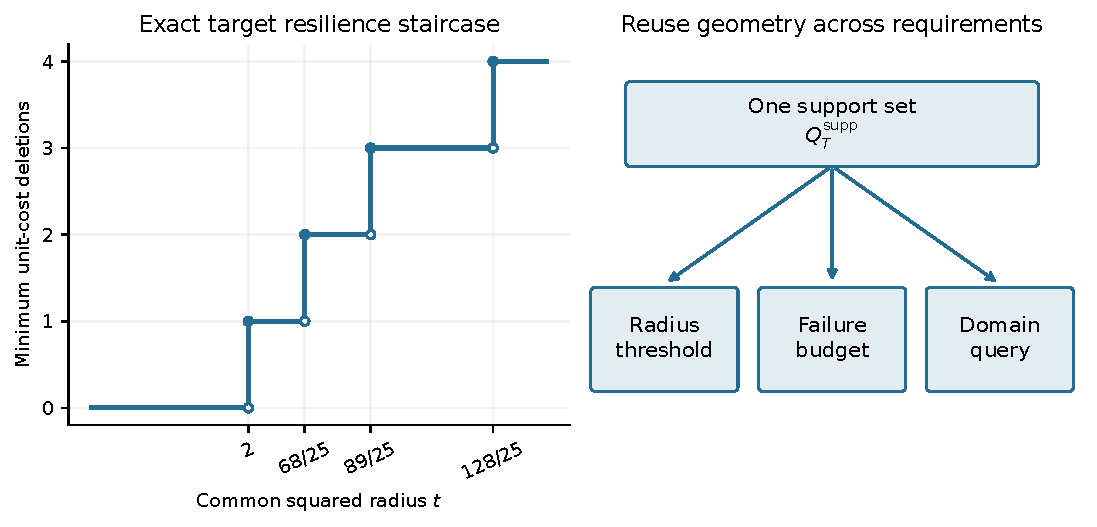
\includegraphics[width=\textwidth]{figures/analytical-frontier.pdf}
\caption{The exact step function in \cref{eq:panel-staircase}. Filled markers indicate accepted equality at each power threshold. The right-hand schematic shows how one support set answers radius, budget and domain queries.}
\end{figure}

\subsection{The resource optimum and the role of duplication}
Each contact occurs in exactly two of the four critical pairs. Under $\sum_i c_i\le1$,
\[
\sum_{A\in\mathcal A_T}c(A)=2\sum_i c_i\le2.
\]
At least one pair therefore has cost at most $1/2$. Uniform allocation $c_i=1/4$ gives cost $1/2$ for every pair. It is optimal, and the uniform distribution on the four cuts is a dual certificate.

Two coincident copies at every corner raise the minimum number of individual unit-cost deletions from two to four. Yet under one fixed linear protection budget, the optimal value stays $1/2$ by \cref{prop:duplication}. No contradiction arises: the unweighted count assumes one cost per copy, whereas the protection problem optimizes total allocated cost under a fixed resource constraint.

Adding a fifth contact at the origin with the same radius $9/5$ gives another distinction. Its disk alone covers the target because $x^2+y^2\le18/25<81/25$. Allocate the full protection budget to that contact to obtain guaranteed deletion cost one. No cut can cost more than the total allocation one, so this is optimal. The bound follows analytically without identifying every new target cut.

\subsection{Wiring and reliability}
Assign the columns to two domains. The left-pair witness depends only on the left domain, and the right-pair witness depends only on the right domain. Both must remain functioning for full target coverage. Assigning the diagonals instead puts one member of every critical pair in each domain, so either domain alone covers the target.

Thus one-domain-loss tolerance fails for column wiring and holds for diagonal wiring. Under independent domain failure probability $p$, reliability is $(1-p)^2$ and $1-p^2$, respectively. The values at $p=1/10$ are $81/100$ and $99/100$. These are exact probabilities in the stated two-domain model. An implementation must justify its domain failure law before interpreting them as hardware reliability.

The exact squared sensing thresholds are $89/25$ for column wiring and $68/25$ for diagonal wiring. Their symbolic derivation in \cref{app:worked} also gives the worst target locations. The nominal $81/25$ lies strictly between them, so the wiring difference changes the accepted design without moving or adding a sensor.

\subsection{Exact uncertainty allowances}
Independent center errors in Euclidean balls of radius $\epsilon$ erode the effective radius to $9/5-\epsilon$ by \cref{cor:erosion}. Two-contact target coverage is therefore robust exactly when
\begin{equation}\label{eq:panel-error}
\epsilon\le\frac{9-\sqrt{68}}5.
\end{equation}
For independent displacement boxes of halfwidth $1/10$, the exact critical squared radius is $157/50$, derived in \cref{app:worked}. Since $157/50<81/25$, the nominal design meets that box-error requirement. The box formula and ball formula are different exact uncertainty supports, not interchangeable numerical tolerances.

\subsection{A three-dimensional sharpness example}
Let the four sites be the vertices
\[
(1,1,1),\quad(1,-1,-1),\quad(-1,1,-1),\quad(-1,-1,1)
\]
of a regular tetrahedron, and let the target be its convex hull. Each site has squared norm three and their centroid is zero. If $x=\sum_i\lambda_i c_i$ is a convex combination of the vertices, then
\begin{equation}\label{eq:tetra-variance}
\sum_i\lambda_i\|x-c_i\|^2=3-\|x\|^2.
\end{equation}
At least one vertex distance squared is therefore at most $3-\|x\|^2$. Away from zero this is strictly less than three. At zero all four distances equal $\sqrt3$. Thus ordinary one-contact coverage has exact radius $\sqrt3$ and its unique worst location is the interior point zero.

All four sites tie there with rank three. No pair or triple of these vertices alone determines the unique three-dimensional equal-distance location. The example shows why the general support theorem allows $d+1$ sites on a $d$-dimensional target. More generally, the same variance identity applies to a cospherical simplex whose center lies in its interior.\footnote{The example shows that the support-size bound cannot generally be reduced from $d+1$ to $d$ by restricting to lower-order equal-distance systems. It is not a lower bound against arbitrary encodings of the target.}

\begin{figure}[!htbp]
\centering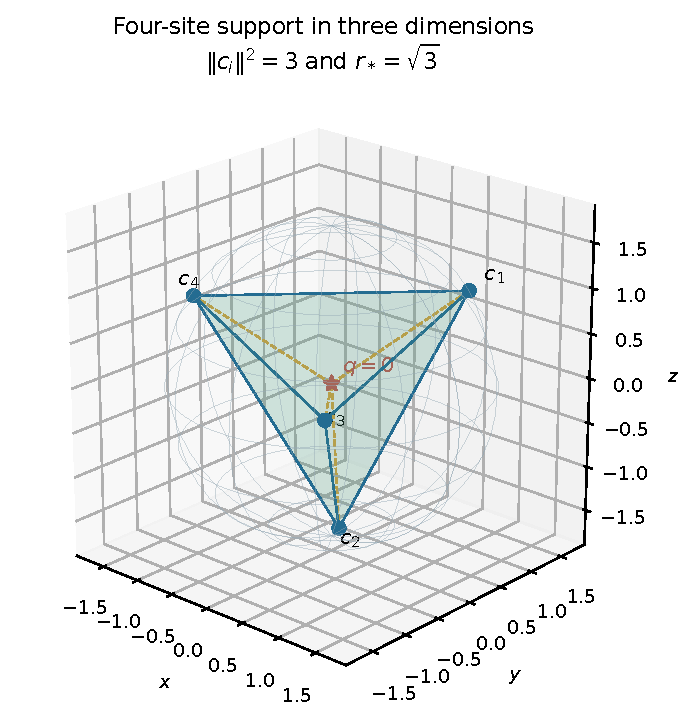
\includegraphics[width=.75\textwidth]{figures/tetrahedron-support.pdf}
\caption{The three-dimensional support example. The tetrahedron, its four sites, the common sphere and the unique worst point illustrate \cref{eq:tetra-variance}. The exact proof is the barycentric identity, not a sampled surface or numerical optimization.}
\end{figure}
\FloatBarrier

\appendix
\section{Order maps and the comparison homotopies}
\label{app:posets}
We spell out the finite order argument used in \cref{thm:duality}. For a poset $P$, its order complex has vertices $p\in P$ and simplices the nonempty chains. An order-preserving map sends chains to chains, possibly with repetitions; deleting repetitions gives a simplicial map. An order-reversing map does the same after reversing the order of the image chain. The order complexes of a poset and its opposite are therefore the same abstract complex.

\begin{lemma}[Order comparison homotopy]\label{lem:order-homotopy}
If $a,b:P\to Q$ are order-preserving maps of finite posets with $a(p)\le b(p)$ for all $p$, their induced maps on realizations are homotopic.
\end{lemma}
\begin{proof}
The map $H:P\times\{0<1\}\to Q$ defined by $H(p,0)=a(p)$ and $H(p,1)=b(p)$ is order preserving. The only mixed comparison needing verification is $(p,0)\le(p',1)$, which implies $p\le p'$ and hence $a(p)\le a(p')\le b(p')$. The order complex of this product triangulates each prism over a chain of $P$: a chain $p_0<\cdots<p_s$ is crossed with an interval and split at each possible transition from level zero to level one. These prism triangulations agree on shared faces. Realizing $H$ gives a continuous homotopy from the realization of $a$ to that of $b$.
\end{proof}

The maps $g f$ and $f g$ of \cref{eq:f-map,eq:g-map} are order preserving and lie above the identity. Applying \cref{lem:order-homotopy} gives both homotopies required there. This avoids choosing a maximal face for each simplex, which would obscure naturality when the failure rule changes.

An alternative intermediate model is the order complex of the winning-face poset $\cP_{\F}$. Define
\[
u:Q_\Gamma\longrightarrow\cP_{\F},\qquad u(A)=\bigcup_{\sigma\in A}\sigma,
\]
and
\[
t:\cP_{\F}\longrightarrow Q_\Gamma,\qquad
t(\sigma)=\{\tau\in\cP_{\F}:\tau\subseteq\sigma\}.
\]
These are order preserving, $u t$ is the identity, and $A\subseteq t u(A)$. Thus $\Gamma_{\F}$ is also homotopy equivalent to the winning-face order complex. For the cardinality rule, this is the subcomplex of the barycentric nerve subdivision on faces of size at least $k$, connecting the present formulation directly to the classical multicover nerve~\cite{sheehy}. The map $u$ commutes with inclusions of winning-face sets at fixed $N$.

\section{A chain comparison for the disk covers}
\label{app:nerve}
This appendix explains the natural homology statement in the semialgebraic disk setting without treating an arbitrary closed cover as an open good cover. A finite family of compact semialgebraic sets admits a common finite compatible triangulation~\cite{realalgebraic,bauer}. Apply this to the finitely many disk intersections appearing in the secondary covers under consideration. Each such set is represented by a subcomplex of a common finite complex $L$. Every nonempty finite intersection remains contractible because it is convex before triangulation.

Index one cover by a finite set $I$, write $L_i$ for its subcomplexes and $L_A=\bigcap_{i\in A}L_i$. Over a field, form the double-chain groups
\begin{equation}\label{eq:double-chain}
E_{p,q}=\bigoplus_{\substack{A\subseteq I\\|A|=p+1}}C_q(L_A),\qquad p,q\ge0,
\end{equation}
omitting empty intersections. The vertical boundary is the simplicial boundary of $L_A$. The horizontal boundary is the alternating sum of inclusions obtained by dropping one index of $A$. The standard total sign convention makes the total differential square to zero; over $\FF$ the signs disappear.

Augment horizontally to the chain complex of the union. For a fixed simplex $s$ of the union, let $I_s=\{i:s\in L_i\}$. This set is nonempty. Its copies in the augmented row of \cref{eq:double-chain} form precisely the augmented chain complex of the full simplex on $I_s$. That complex is exact: fixing one index in $I_s$ and adjoining it gives a contracting homotopy. Splitting the row over the simplices $s$ proves horizontal exactness. Thus the total chain complex computes the homology of the union.

In the other direction, take vertical homology first. Each nonempty $L_A$ is contractible, so it has one-dimensional ordinary $H_0$ and zero higher homology. Sending every vertex of a connected $L_A$ to $1$ identifies its $H_0$ with the coefficient field compatibly with inclusion. The remaining horizontal complex is exactly the simplicial chain complex of the nerve. The two filtrations of the finite double complex therefore identify nerve homology with union homology. This can be expressed as the two elementary finite spectral-sequence comparisons, or by successive elimination of the exact augmented rows and the positive-degree acyclic columns.

If a cover subfamily is included in a larger cover, the same triangulation can be used for both, and inclusion of summands in \cref{eq:double-chain} commutes with both augmentations. Hence the resulting homology isomorphisms are natural. No human choice of one witness point per nerve simplex enters the induced homology comparison. The general closed-convex homotopy theorem used in \cref{thm:duality} is the standard theorem cited in~\cite{bauer}; this appendix supplies a detailed homological explanation for the disks actually computed.

\section{Boundary arithmetic and exact input semantics}
\label{app:arithmetic}
\subsection{Binary columns over \texorpdfstring{$\FF$}{F2}}
Number the dual edges from zero to $E-1$. A triangle with edge indices $a,b,c$ has boundary column
\[
z=2^a\mathbin{\oplus}2^b\mathbin{\oplus}2^c,
\]
where $\oplus$ is bitwise exclusive-or. This is simply an encoding of a vector in $\FF^E$; it is not integer linear algebra. Each edge has two vertex endpoints, so applying the edge boundary to a triangle boundary counts every vertex twice. Therefore $\partial_1\partial_2=0$.

To compute the rank, maintain at most one pivot column for each leading nonzero row. A new column is repeatedly added to the stored column with the same leading row until it becomes zero or acquires a previously unused leading row. In the latter case store it. Every reduction step preserves the span of columns seen so far. Stored columns have distinct leading rows and are linearly independent. Each processed column is in their span, so the number stored is exactly the boundary rank. Termination follows because the leading nonzero row strictly decreases in the main implementation.

One may instead represent columns by sets and use the smallest nonzero row. That leading row strictly increases. The same span invariant proves correctness for every finite input, independently of the chosen representation or pivot direction.

\subsection{Rational comparisons and equality}
A finite binary64 number is a rational of the form $m2^e$. The input conversion preserves that value as a Python \texttt{Fraction}. Products, sums and divisions in \cref{eq:circle-parameters,eq:quadratic-membership,eq:mec} therefore have exact integer numerators and denominators. The only radicals are eliminated by the signed comparisons of \cref{lem:sign}. Unconditional squaring would be wrong when the compared sides have uncontrolled signs; the sign cases are part of the algorithm.

The geometry API explicitly converts supplied numerical values to binary64 before making their rational representations. Passing a rational with a non-dyadic denominator to that API does not request symbolic preservation of the original rational; it requests exact treatment of its binary64 conversion. The abstract rational algorithm of \cref{thm:algorithm} can instead be implemented with rational inputs directly. The rational analytical statements are independent of either software input convention.

No geometric epsilon is used to merge circles, enlarge radii or decide tangency. Equal centers are tested as exact rational pairs. Coincident disks retain distinct labels because a failure model can distinguish the two contacts even when their geometry is identical. Equality in a closed-disk test is accepted. The companion archive's open-disk routines~\cite{ecog} use strict inequalities, so they must not be interchanged without specifying the convention.

\section{Counterexamples to stronger interpretations}
\label{app:counterexamples}
\begin{example}[Hole-free does not imply target coverage]
Let $D_1$ be the unit disk at the origin and let the target be the unit disk centered at $(10,0)$. The ordinary covered region is contractible and has $b_1=0$, but its intersection with the target is empty. No theorem using only the absolute Betti numbers of the covered region can certify containment of every possible externally supplied target.
\end{example}

\begin{example}[Pairwise overlap does not determine a triangle]
Three disks centered at the vertices of an equilateral triangle of side $d$ overlap pairwise when $r\ge d/2$, but share a common point only when $r\ge d/\sqrt3$. For $d/2<r<d/\sqrt3$, their nerve contains a cycle without a filled triangle. Replacing the nerve by the flag complex of pairwise overlaps changes $H_1$. The same issue appears again in the facet-intersection model, as noted after \cref{prop:two-skeleton}.
\end{example}

\begin{example}[Geometric uncertainty can hide temporary homology]
Even when an inner region and an outer region are both disks, an intermediate subset containing the inner disk and contained in the outer disk can be an annulus attached to that disk, or a disk with a separate small component. Thus knowledge of endpoint Betti numbers alone does not determine all intermediate Betti numbers. The rank lower bound after \cref{thm:stability} is the conclusion that follows from the factorization; a stronger exactness assertion would require additional hypotheses.
\end{example}

\section{Finite minimax and rational protection certificates}
\label{app:minimax}
We give the finite minimax argument used in \cref{thm:protection}. This is a classical duality principle. The proof is included to make the verification inequalities and their attainment transparent.

\begin{lemma}[Finite matrix minimax]
For any real $m\times n$ matrix $B$,
\[
\max_{x\in\Delta_n}\min_{a\in[m]}(Bx)_a
=\min_{\lambda\in\Delta_m}\max_{i\in[n]}(\lambda^TB)_i.
\]
\end{lemma}
\begin{proof}
Call the left value $v$. For every $x$ and $\lambda$, the minimum coordinate of $Bx$ is at most $\lambda^TBx$, which is at most the maximum coordinate of $\lambda^TB$. This gives the weak inequality.

For the converse, let $P$ be the convex hull of the columns of $B$, and fix $t>v$. The compact convex set $P$ is disjoint from $K_t=\{u\in\R^m:u_a\ge t\text{ for all }a\}$. Their distance is positive and is attained at a pair $(z_0,u_0)$. Indeed, distance to a closed set is continuous on compact $P$, and the nearest point in $K_t$ to a given $z$ is obtained by replacing each coordinate below $t$ by $t$.

Put $b=u_0-z_0\ne0$. First-order comparison of squared distances along segments in $P$ and $K_t$ gives
\[
b\cdot z\le b\cdot z_0\quad(z\in P),\qquad
b\cdot u\ge b\cdot u_0\quad(u\in K_t).
\]
Since $K_t$ contains $u_0+s e_a$ for $s\ge0$, each $b_a\ge0$. Normalize $\lambda=b/(\sum_a b_a)$. Then $\lambda\in\Delta_m$. The separating inequalities are strict between $z_0$ and $u_0$, because their scalar-product difference is $\|b\|^2>0$. The minimum of $\lambda\cdot u$ on $K_t$ is $t$, so
\[
\max_i(\lambda^TB)_i=\max_{z\in P}\lambda\cdot z<t.
\]
Take a sequence $t\downarrow v$ and use compactness of $\Delta_m$ and continuity of the finite coordinate maximum. A limiting $\lambda$ gives dual value at most $v$, proving the reverse inequality and attainment.
\end{proof}

For rational protection data, the primal can be restricted to a bounded rational polytope by using $c_i\le C/d_i$ and $0\le t\le C/\min_i d_i$. A maximizing face has a vertex obtained by solving independent active constraints, so a rational optimum exists. The dual has a rational optimal vertex after imposing any known feasible upper bound on $\mu$. Rational certificates are therefore appropriate exact objects for this model, although recovering them from a numerical hint may fail in a particular implementation.

\subsection{A checker independent of the LP solver}
Given a cut list and rational arrays $c$, $\lambda$, $d$ and numbers $C,\mu$, a checker verifies:
\begin{enumerate}
\item $c_i\ge0$, $d_i>0$, $\sum_i d_i c_i\le C$;
\item $\lambda_A\ge0$ and $\sum_A\lambda_A=1$;
\item $\sum_{A\ni i}\lambda_A\le\mu d_i$ for every contact;
\item $\min_A c(A)=C\mu$.
\end{enumerate}
The weak-duality chain in \cref{thm:protection} proves optimality from these finite checks. The checker need not trust a simplex basis, floating-point tolerance or solver implementation. It does depend on the completeness of the geometric cut list, which is justified separately by \cref{thm:sweep} or \cref{cor:all-radii}.

\section{Direct derivations for the four-corner panel}
\label{app:worked}
Let $a=3/5$, let $T=[-a,a]^2$, and place the four sites at $(\pm1,\pm1)$. For a target point write $u=\max\{|x|,|y|\}$ and $v=\min\{|x|,|y|\}$. Then $0\le v\le u\le a$. The ordered squared distances are
\begin{align*}
d_1^2&=2+u^2+v^2-2u-2v,\\
d_2^2&=2+u^2+v^2-2u+2v,\\
d_3^2&=2+u^2+v^2+2u-2v,\\
d_4^2&=2+u^2+v^2+2u+2v.
\end{align*}
Each is convex on the triangle with vertices $(0,0)$, $(a,0)$ and $(a,a)$, so its maximum there is attained at a vertex. It follows that
\[
\max_T d_1^2=2,\qquad
\max_T d_2^2=2+2a^2=68/25,
\]
\[
\max_T d_3^2=2+2a+a^2=89/25,\qquad
\max_T d_4^2=2+4a+2a^2=128/25.
\]
These give all four contact thresholds independently of the support algorithm, including every step of \cref{eq:panel-staircase}.

At any generic target point the two nearest corners share an edge. At a tie, the active group contains such a pair. Since $(9/5)^2>68/25$, every active set at nominal radius $9/5$ contains an adjacent pair. At $(-11/20,0)$ the squared distances to the left corners are $481/400$, while those to the right corners are $1361/400$. They lie on opposite sides of $81/25=1296/400$, giving exactly the left pair. The three symmetric locations give the other adjacent pairs. This proves \cref{eq:panel-cuts} directly.

\subsection{Column and diagonal domains}
To tolerate a column-domain loss, either column alone must cover $T$. The farthest target point from the nearer site in a surviving column is the midpoint of the opposite target edge. Its squared distance is $(1+a)^2+1=89/25$.

For the diagonal containing $(1,1)$ and $(-1,-1)$, the nearer squared distance is
\[
2+x^2+y^2-2|x+y|.
\]
On each side of the line $x+y=0$ this is a squared norm to one fixed corner, hence convex. Its maximum over the two triangular halves of $T$ occurs at their vertices, giving $2+2a^2=68/25$. The other diagonal has the same value. These calculations prove the distinct domain thresholds directly.

\subsection{Box displacement uncertainty}
Give every site independent coordinate errors in $[-b,b]^2$ with $b=1/10$. Throughout $T$, the farthest allowed center for a corner site is its outward shifted corner $(\pm(1+b),\pm(1+b))$. This follows coordinatewise because target coordinates stay strictly between the nominal corner coordinates. Thus, restricted to $T$, the guaranteed distance for each physical contact is the distance to that one outward center.

Repeating the ordered-distance calculation with corner magnitude $1+b$ gives the two-contact critical square
\[
2(1+b)^2+2a^2=2(11/10)^2+2(3/5)^2=157/50.
\]
This independently verifies the sixteen-primitive bundle computation. The reduction to one outward corner is special to this target's position inside the nominal square; the general uncertainty algorithm keeps all four box vertices.

\subsection{The three target patches}
For the three-asset example, the farthest point of each triangular patch from either of its two intended centers is one of the patch vertices, by convexity of squared distance. Direct substitution gives values below $(6/5)^2$. At the patch about $(0,0)$, every point has distance at least $3/2-\sqrt2/20>6/5$ from the third center. At the other patches the corresponding pair midpoint has distance $\sqrt{45}/4$ from the excluded center, and subtracting $\sqrt2/20$ still exceeds $6/5$. Hence each patch has exactly its intended pair of active contacts. The three masks and odd-cycle obstruction follow.

The exact state reliability is $1-3p^2+2p^3$. The protection allocation and dual distribution both equal $(1/3,1/3,1/3)$, with value $2/3$. Thus the geometry, coloring, reliability and optimization conclusions for this example each have a direct derivation as well as an executable control.

\section{Support degeneracies and boundary conventions}
\label{app:support-degeneracy}
\subsection{Coincident sites}
Coincident physical contacts have equal distance functions everywhere but can have different failure labels. The support proof groups their equal geometric positions while retaining every label in the winning predicate. A collection of coincident sites supplies no independent bisector equations. If fewer than $f$ independent restricted differences occur at a candidate maximizer on an $f$-face, the tangent-direction contradiction in \cref{thm:support-radius} still applies.

\subsection{Collinear triples}
In the plane, three distinct collinear centers cannot all be at the same distance from a point, since a circle meets a line in at most two points. They therefore do not determine a finite circumcenter and are skipped by the support construction. A nonsingular triple uses two exact linear equations. Near-collinearity changes rational denominator sizes but does not justify replacing the determinant by a tolerance.

\subsection{An edge coinciding with a bisector}
If a target edge lies on a site-pair bisector, that equality gives no isolated support point on the edge. Along it, the two distances remain equal and their common square is a strictly convex quadratic in an edge parameter. A relative interior maximum therefore requires a further threshold tie, or else occurs at an endpoint. The extra tie yields a triple support; the endpoints are already supplied target vertices. This is the rank test in \cref{thm:support-radius}, not a missing numerical special case.

\subsection{Why open footprints change the fixed-radius question}
For closed footprints, coverage at the critical common radius is accepted: $r\ge r_w^*$. With open disks, equality may fail at a maximizing witness. Moreover, interior-cell masks alone need not describe coverage of all target boundary points by open sets. The vertical target theorem and its closed-set witness lemma are therefore not silently transferred to strict inequalities.

\subsection{Why lower-dimensional targets need their own strata}
An isolated target point on a disk tangency can have an active mask absent from every two-dimensional cell. A target containing a line segment as a separate appendage can have the same issue on that segment. The regular-closed target hypothesis excludes these cases from the full-dimensional sweep. The common-radius support theorem itself can be applied face by face to prescribed simplices of the appropriate dimension, but that is a different stratified input specification.

\section*{Declarations}

\noindent\textbf{Funding.} None.

\noindent\textbf{Competing interests.} None.

\noindent\textbf{Ethics.} Not applicable; the article contains no research involving human participants or animals.

\noindent\textbf{Data availability.} The \LaTeX{} source and the finite checks of the worked examples are archived in the repository \url{https://github.com/creelie/sensor-resilience-certificates}, release \releaseTag, on Zenodo at \href{https://doi.org/\zenodoCodeID}{doi:\zenodoCodeID}. No statement of the paper depends on them. OpenAI Codex and Anthropic Claude assisted with exposition, figures and the finite checks; the authors checked every proof and are responsible for the text.

\begin{thebibliography}{99}\raggedright
\bibitem{original}
D.~Bhattacharjee and U.~Bhattacharya,
\emph{Iterated Nerve Complexes for $k$-Fold Sensor Coverage},
Preprints.org, version 2, 2026.
\href{https://doi.org/10.20944/preprints202606.1351.v2}{doi:10.20944/preprints202606.1351.v2}.

\bibitem{ecog}
A.~Bose, D.~Bhattacharjee and U.~Bhattacharya,
\emph{Certified Redundant ECoG Coverage: Exact Geometry, Continuous Mesh Certificates and Reproducible Audits},
research and software archive, version 1.6.0, Zenodo, 2026.
\href{https://doi.org/10.5281/zenodo.23731783}{doi:10.5281/zenodo.23731783}.

\bibitem{sheehy}
D.~R.~Sheehy,
\emph{A multicover nerve for geometric inference},
Proceedings of the 24th Canadian Conference on Computational Geometry, Charlottetown, 2012.
\url{https://mathtube.org/sites/default/files/lecture-notes/e-proceedings.pdf}.

\bibitem{corbet}
R.~Corbet, M.~Kerber, M.~Lesnick and G.~Osang,
\emph{Computing the multicover bifiltration},
Discrete Comput. Geom. \textbf{70} (2023), 376--405.
\href{https://doi.org/10.1007/s00454-022-00476-8}{doi:10.1007/s00454-022-00476-8}.

\bibitem{alonso}
\'{A}.~J.~Alonso,
\emph{A sparse multicover bifiltration of linear size},
Discrete Comput. Geom., published online August 4, 2026.
\href{https://doi.org/10.1007/s00454-026-00865-3}{doi:10.1007/s00454-026-00865-3}.

\bibitem{dowker}
C.~H.~Dowker,
\emph{Homology groups of relations},
Ann. of Math. (2) \textbf{56} (1952), 84--95.
\href{https://doi.org/10.2307/1969768}{doi:10.2307/1969768}.

\bibitem{chowdhury}
S.~Chowdhury and F.~M\'emoli,
\emph{A functorial Dowker theorem and persistent homology of asymmetric networks},
J. Appl. Comput. Topol. \textbf{2} (2018), 115--175.
\href{https://doi.org/10.1007/s41468-018-0020-6}{doi:10.1007/s41468-018-0020-6}.

\bibitem{bauer}
U.~Bauer, M.~Kerber, F.~Roll and A.~Rolle,
\emph{A unified view on the functorial nerve theorem and its variations},
Expo. Math. \textbf{41} (2023), no.~4, article 125503.
\href{https://doi.org/10.1016/j.exmath.2023.04.005}{doi:10.1016/j.exmath.2023.04.005}.

\bibitem{ghrist}
R.~Ghrist and A.~Muhammad,
\emph{Coverage and hole-detection in sensor networks via homology},
Proceedings of IPSN 2005, IEEE, 2005, 254--260.

\bibitem{desilva}
V.~de Silva and R.~Ghrist,
\emph{Coverage in sensor networks via persistent homology},
Algebr. Geom. Topol. \textbf{7} (2007), 339--358.
\href{https://doi.org/10.2140/agt.2007.7.339}{doi:10.2140/agt.2007.7.339}.

\bibitem{controlled}
V.~de Silva and R.~Ghrist,
\emph{Coordinate-free coverage in sensor networks with controlled boundaries via homology},
Int. J. Robot. Res. \textbf{25} (2006), 1205--1222.

\bibitem{realalgebraic}
J.~Bochnak, M.~Coste and M.-F.~Roy,
\emph{Real Algebraic Geometry},
Ergebnisse der Mathematik und ihrer Grenzgebiete (3), vol.~36, Springer, Berlin, 1998.
\href{https://doi.org/10.1007/978-3-662-03718-8}{doi:10.1007/978-3-662-03718-8}.

\bibitem{topoi}
D.~Bhattacharjee,
\emph{Neuromorphic Grothendieck topoi for grid-embedded circuit architectures},
SSRN, 2026.
\href{https://doi.org/10.2139/ssrn.6194939}{doi:10.2139/ssrn.6194939}.

\bibitem{suspension}
D.~Bhattacharjee,
\emph{Suspension of structures in two-dimensional topologies with or without the presence of $\mathcal X\ge1$ genus deformations for canonical $2^{2\eta}$ stabilizer points},
Research Square, version 1, 2022.
\href{https://doi.org/10.21203/rs.3.rs-1798323/v1}{doi:10.21203/rs.3.rs-1798323/v1}.

\bibitem{linkage}
S.~Singha Roy, D.~Bhattacharjee and R.~Sadhu,
\emph{Instability in the linkage of topological spaces due to background ghosts},
EPRA Int. J. Res. Dev. \textbf{8} (2023), no.~4, 276--279.
\href{https://doi.org/10.36713/epra13019}{doi:10.36713/epra13019}.

\bibitem{arrangements}
E.~Fogel, D.~Halperin and R.~Wein,
\emph{CGAL Arrangements and Their Applications: A Step-by-Step Guide},
Geometry and Computing, vol.~7, Springer, 2012.
\href{https://doi.org/10.1007/978-3-642-17283-0}{doi:10.1007/978-3-642-17283-0}.

\bibitem{coverage2003}
C.-F.~Huang and Y.-C.~Tseng,
\emph{The coverage problem in a wireless sensor network},
Proceedings of WSNA 2003, ACM, 2003, 115--121.

\bibitem{integrated}
X.~Wang, G.~Xing, Y.~Zhang, C.~Lu, R.~Pless and C.~Gill,
\emph{Integrated coverage and connectivity configuration in wireless sensor networks},
Proceedings of SenSys 2003, ACM, 2003, 28--39.

\bibitem{barlow}
R.~E.~Barlow and F.~Proschan,
\emph{Statistical Theory of Reliability and Life Testing: Probability Models},
Holt, Rinehart and Winston, New York, 1975.

\bibitem{polychromatic}
B.~Bollob\'as, D.~Pritchard, T.~Rothvoss and A.~Scott,
\emph{Cover-decomposition and polychromatic numbers},
SIAM J. Discrete Math. \textbf{27} (2013), no.~1, 240--256.
\href{https://doi.org/10.1137/110856332}{doi:10.1137/110856332}.

\bibitem{lattice}
J.-L.~Marichal,
\emph{Weighted lattice polynomials},
Discrete Math. \textbf{309} (2009), no.~4, 814--820.
\href{https://doi.org/10.1016/j.disc.2008.01.019}{doi:10.1016/j.disc.2008.01.019}.

\bibitem{reliability-lattice}
A.~Dukhovny and J.-L.~Marichal,
\emph{System reliability and weighted lattice polynomials},
Probab. Engrg. Inform. Sci. \textbf{22} (2008), no.~3, 373--388.
\href{https://doi.org/10.1017/S0269964808000223}{doi:10.1017/S0269964808000223}.

\bibitem{robustbook}
A.~Ben-Tal, L.~El Ghaoui and A.~Nemirovski,
\emph{Robust Optimization},
Princeton University Press, Princeton, 2009.
\href{https://doi.org/10.1515/9781400831050}{doi:10.1515/9781400831050}.

\bibitem{hailperin}
T.~Hailperin,
\emph{Best possible inequalities for the probability of a logical function of events},
Amer. Math. Monthly \textbf{72} (1965), no.~4, 343--359.
\href{https://doi.org/10.1080/00029890.1965.11970533}{doi:10.1080/00029890.1965.11970533}.

\bibitem{csikos}
B.~Csik\'os,
\emph{On the volume of flowers in space forms},
Geom. Dedicata \textbf{86} (2001), 59--79.
\href{https://doi.org/10.1023/A:1011983123985}{doi:10.1023/A:1011983123985}.

\bibitem{aurenhammer}
F.~Aurenhammer,
\emph{Power diagrams: properties, algorithms and applications},
SIAM J. Comput. \textbf{16} (1987), no.~1, 78--96.
\href{https://doi.org/10.1137/0216006}{doi:10.1137/0216006}.
\bibitem{toussaint}
G.~T.~Toussaint,
\emph{Computing largest empty circles with location constraints},
Int. J. Comput. Inf. Sci. \textbf{12} (1983), no.~5, 347--358.
\href{https://doi.org/10.1007/BF01008046}{doi:10.1007/BF01008046}.

\bibitem{leekvoronoi}
D.-T.~Lee,
\emph{On $k$-nearest neighbor Voronoi diagrams in the plane},
IEEE Trans. Comput. \textbf{C-31} (1982), no.~6, 478--487.
\href{https://doi.org/10.1109/TC.1982.1676031}{doi:10.1109/TC.1982.1676031}.

\bibitem{soye}
A.~M.-C.~So and Y.~Ye,
\emph{On solving coverage problems in a wireless sensor network using Voronoi diagrams},
in: Internet and Network Economics (WINE 2005), Lecture Notes in Comput. Sci., vol.~3828, Springer, Berlin, 2005, 584--593.
\href{https://doi.org/10.1007/11600930_58}{doi:10.1007/11600930\_58}.
\end{thebibliography}

\end{document}
